\chapter{Stand van zaken}
\label{ch:stand-van-zaken}
In dit hoofdstuk wordt een literatuurstudie gevoerd naar blockchain-gebaseerde stemsystemen en hun potentieel. Daar dit een vrij complex onderwerp is, wordt dit hoofdstuk onderverdeeld in drie logische segmenten.

 Deel 1 vormt een inleiding tot de blockchain-technologie: Door het bespreken van de fundamentele concepten en achterliggende filosofie  maakt de  lezer kennis  met  blockchain. Dit alles wordt gedaan aan de hand van \textcite{Nakamoto2008}, de grondlegger van blockchain als technologie.  Hoewel de concepten die aan bod komen enigszins gedateerd zijn, zijn ze -op conceptueel niveau- noodzakelijk voor al wie deze technologie wil aanwenden.

In deel 2 worden het Ethereum platform en smart-contracts besproken. Waar deel 1 over de Bitcoin-blockchain handelt, bespreekt deel 2  Ethereum. Zo krijgt de lezer een inleiding in 's werelds tweede populairste blockchain-netwerk. De focus ligt echter niet op Ethereum omdat het één van de grootste of de populairste onder de blockchains is, maar omdat het één van de meest vooruitstrevende is, vooral op het vlak van \textit{smart-contracts}. Het begrijpen van de werking en het potentieel van deze `contracten' zal ontzettend van pas komen tijdens de implementatie van een blockchain-gebaseerd stemsysteem, in het volgende hoofdstuk.

In deel 3 wordt tot slot blockchain-gebaseerd stemmen besproken. Na algemene kennis over blockchain-concepten en specifieke kennis over de werking van Ethereum en smart-contracts, krijgt de lezer nu ook een inzicht in de mogelijkheden van de technologie. Dit finale deel van de literatuurstudie behandelt blockchain-gebaseerd stemmen volledig: van noodzaak over verschillende implementaties, tot de achterliggende cryptografie die nodig is om zelf een implementatie te schrijven. Ook de voor- en nadelen van blockchain-gebaseerd stemmen komen aan bod.

\newpage
\section{Blockchain}
	\subsection*{Inleiding}
	In het eerste deel van dit hoofdstuk wordt de blockchain-technologie in haar basisvorm besproken. We beginnen met het introduceren van de verschillende concepten en principes waarop blockchain gebouwd is.  We doen dit door het bespreken van datgene wat \textcite{Swan2015} blockchain 1.0 noemt, ofwel de Bitcoin-blockchain. In het paper `Bitcoin: A Peer-to-Peer Electronic Cash System' beschrijft de auteur, onder het pseudoniem `Satoshi Nakamoto' een monetair systeem dat niet verbonden is aan een bank of  andere financiële institutie. Nakamoto is de oorspronkelijke ontwerper van de Bitcoin en richtte de eerste blockchain-database op. Tot vandaag blijft de ware identiteit van deze persoon (of entiteit) een mysterie. Het paper werd gepubliceerd op 31 oktober 2008 en wordt vandaag gezien als het blockchain white paper. De structuur beschreven door \textcite{Nakamoto2008} vormde de basis voor wat men vandaag blockchain noemt.
	\subsection{Noodzaak}
			\subsubsection{Vertrouwen in plaats van bewijs}
			\textcite{Nakamoto2008} start met de vaststelling dat het verkopen van waren en diensten op het internet zo goed als volledig afhankelijk is van grote financiële instituties, die optreden als derde partij voor het verwerken van elektronische transacties. 
		
			Hoewel ons huidige betaalmodel naar behoren werkt voor de meeste transacties, kent het volgens de auteur van het paper toch een inherent zwaktepunt: het is namelijk een systeem dat gebaseerd is op vertrouwen en niet op bewijs.
			
			Transacties in het huidige systeem, zo stelt \textcite{Nakamoto2008}, zijn namelijk niet definitief: een pas uitgevoerde transactie is in veel gevallen nog omkeerbaar. Voor de financiële instellingen die fungeren als derde partij kan dit ook niet anders: het is onvermijdelijk dat geschillen zullen optreden over bepaalde transacties. Bijgevolg is het ook onvermijdelijk dat er situaties zullen zijn waarin de instellingen moeten ingrijpen door transacties ongedaan te maken. Omdat transacties in het huidige systeem niet als definitief kunnen beschouwd worden, is er een zekere graad van vertrouwen nodig om een transactie aan te gaan tussen de betrokken partijen, vooral voor de ontvangende partij. 
			
			\textcite{Nakamoto2008} geeft hier het voorbeeld van online-verkopers die zich genoodzaakt zien om hun klanten om meer persoonlijke informatie te vragen dan ze eigenlijk nodig hebben. En ook al worden er meer gegevens gevraagd dan nodig, dan nog is een zeker fraudepercentage onvermijdbaar. 
		
			Wanneer men de analogie maakt naar het gebruik van cash, dan ziet men dat de bovenstaande problemen in veel mindere mate voorkomen. Bij het gebruik van cash gebeurt de transactie immers niet enkel op basis van vertrouwen, maar vooral op basis van wederzijdse controle. Als een klant een bepaald bedrag betaalt of wisselgeld ontvangt, dan wordt het geld geteld ter controle. Idem dito voor de ontvangende kant. Bij cash is het minder evident om een transactie ongedaan te maken. 
			
			\textcite{Nakamoto2008} komt tot de conclusie dat een alternatief elektronisch betalingssysteem nodig is. In zo’n systeem zouden transacties niet mogen gebeuren op basis van vertrouwen, maar eerder op basis van wederzijdse controle, net zoals bij het voorbeeld van cash. Een op cryptografisch bewijs gebaseerd controlemechanisme zou twee partijen in staat kunnen stellen om online-transacties rechtstreeks met elkaar aan te gaan, zonder daarbij gebruik te moeten maken van een vertrouwde derde partij. De noodzaak tot een financiële instantie zoals een bank, is in een dergelijk systeem dus volledig geëlimineerd.
		
			In het systeem dat \textcite{Nakamoto2008} voorstelt, zijn de transacties beschermd door cryptografie die het computationeel onpraktisch maakt om ze ongedaan te maken. De transacties zijn praktisch onomkeerbaar en beschermen hiermee verkopers tegen fraude. Bovendien zijn borgmechanismen nodig om ook kopers te beschermen. Deze zijn volgens de auteur ook makkelijk te implementeren in het systeem.
			
			\subsubsection{Het double-spending probleem}
			 \textcite{Nakamoto2008} schenkt veel aandacht aan het oplossen van het double-spending probleem. Dit probleem beschrijft het bestaande risico dat - bij een digitale vorm van geld of een ander digitaal middel - dezelfde middelen meerdere malen gespendeerd kunnen worden.
			
			Een van de fundamentele verschillen tussen contant en elektronisch geld is dat het eerste van fysieke aard is. Dat betekent dat geld tastbaar is, men draagt het bij zich en geeft het door bij transacties. Het geld veranderd van eigenaar en kan niet opnieuw aangewend worden. Er is geen bank of andere financiële instantie nodig om dit te verifiëren. Hoeveel men spendeert en hoeveel vermogen er nog rest is evident. 
			
			Bij elektronische betaalmiddelen is dit alles veel complexer. Ter verduidelijking nemen we hier het voorbeeld van een klassieke rekening bij een bank.
			
			\begin{figure}
				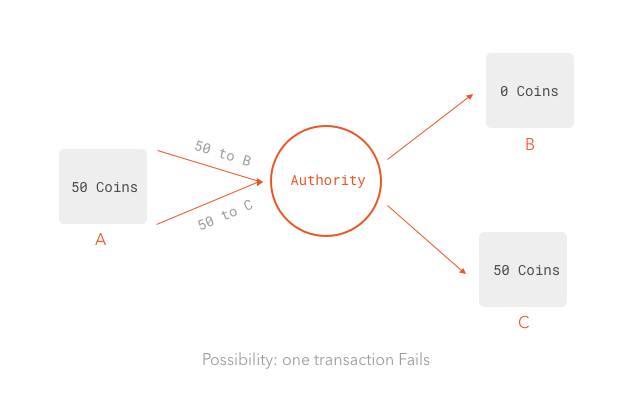
\includegraphics[width=\linewidth]{img/double_spending2.png}
				\caption{Double-spending bemoeilijkt door een centrale autoriteit}
				\label{fig:double_spending2}
			\end{figure}
			
			 Geld op de hedendaagse bankrekening bestaat enkel en alleen als een elektronisch getal: een reeks van digitale cijfers bestaande uit 1’en en 0’en. Zo’n getal op zichzelf is gemakkelijk te wijzigen, men hoeft slechts enkele 1’en en 0’en toe te voegen om een veelvoud van het oorspronkelijke te bekomen. Het is de bank die instaat voor de beveiliging van elektronisch geld. Waar de bank van weleer de bewaker was van vermogens in de vorm van kluizen of goudreserves, is de bank van vandaag de digitale bewaker van binaire vermogens.
			
			Bij een typische elektronische transactie tussen twee partijen, vindt er geen transfer van fysieke objecten plaats, maar een verlaging van het elektronische vermogen van de eerste partij en een verhoging van het vermogen van de tweede. 
		
			Gezien de enorme complexiteit die de beveiliging van digitale systemen met zich meebrengt, is het uitvoeren van elektronische transacties binnen het klassieke monetaire systeem altijd de verantwoordelijkheid van een vertrouwde derde partij geweest. Wanneer men een elektronische aankoop doet, is het deze derde partij die een centrale autoriteit vormt wat betreft de veiligheid en de geldigheid van de transactie. Het is de vertrouwde derde partij die controleert op double-spending, vervolgens een bepaald bedrag in mindering brengt van het oorspronkelijke vermogen en dit bedrag tenslotte toevoegt aan de kant van de verkoper. Dit wordt geïllustreerd in figuur \ref{fig:double_spending2}.
			
			In de meeste gevallen neemt de vertrouwde derde partij de vorm aan van een bank, maar ook alternatieve instanties kunnen optreden als vertrouwde derde partij voor transacties. Voorbeelden hiervan zijn PayPal, TransferWise, Google Pay en Apple Pay.
		
			Haalt men deze derde partij echter volledig uit het proces, dan dringt de nood voor een compleet nieuwe oplossing voor het double-spending probleem zich onmiddellijk op.  Dit wordt geïllustreerd in figuur \ref{fig:double_spending1}.
			
			\begin{figure}
				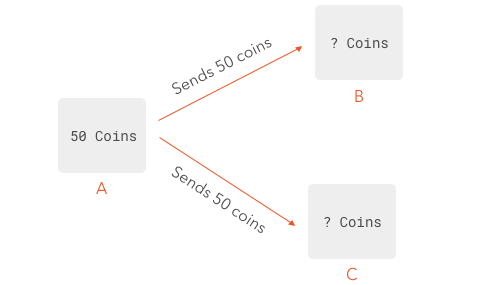
\includegraphics[width=\linewidth]{img/double_spending1.png}
				\caption{Double-spending zonder centrale autoriteit}
				\label{fig:double_spending1}
			\end{figure}
		
			Double-spending vormt een dusdanig groot probleem dat  de ontwikkeling van elektronisch geld zonder een vertrouwde autoriteit lange tijd onmogelijk werd geacht. In de volgende secties wordt de oplossing van \textcite{Nakamoto2008} voor dit probleem besproken. 
			
			\subsubsection{Het Byzantijnse generaalsprobleem}
			Het double-spending probleem is specifiek is voor digitale valuta. Het Byzantijnse generaalsprobleem is gelijkaardig, alleen is het van toepassing op een iets bredere context. Het Byzantijnse vraagstuk omschrijft namelijk het achterliggende probleem bij double-spending: de vraag hoe men vertrouwen achterwege laat in een systeem zonder centrale autoriteit.
			
			Het probleem luidt als volgt: generaals van Byzantium moeten hun troepen coördineren voor een aanval, en dit op basis van berichten die ze naar elkaar versturen. De aanval moet met meer dan de helft van het totaal aantal troepen op een exact moment worden uitgevoerd, anders zal deze falen. Het is echter mogelijk dat een of meerdere generaals verraders zijn, die de aanval willen dwarsbomen. De identiteit van deze generaals kan echter niet achterhaald worden. De probleemstelling is daarom: hoe kunnen de generaals die te goeder trouw zijn toch hun troepen coördineren voor de aanval, vrij en open met elkaar communicerend, zonder dat een verrader hun plannen kan dwarsbomen door valse berichten te versturen? Het Byzantijnse generaalsprobleem wordt geillustreerd door figuur \ref{fig:byzantium}
			
			Het Byzantijnse generaalsprobleem is tot op vandaag erg relevant, omdat het van toepassing is op eender welke context waarin communicatie tussen verschillende entiteiten een cruciale rol speelt en er geen absoluut vertrouwen is. Het gebied van gedistribueerde computernetwerken is hier een perfect voorbeeld van. De oplossing van \textcite{Nakamoto2008} claimt niet alleen het double-spending probleem op te lossen, maar ook het Byzantijnse generaalsprobleem. Men spreekt ook wel van een model met Byzantijnse fouttolerantie.
			
			\begin{figure}
				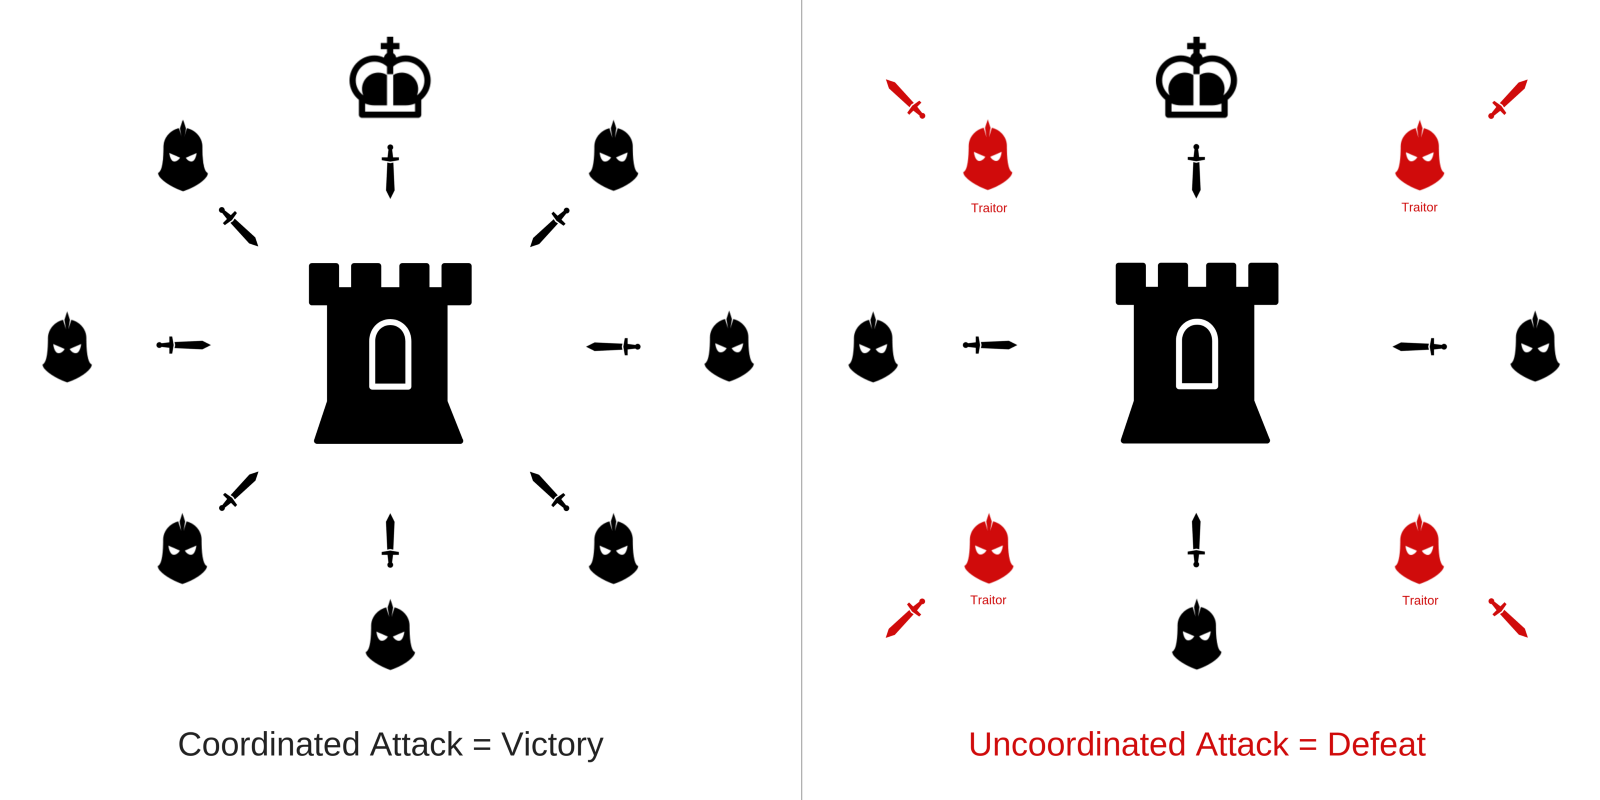
\includegraphics[width=\linewidth]{img/byzantine_generals.png}
				\caption{Het Byzantijnse generaalsprobleem}
				\label{fig:byzantium}
			\end{figure}
			
	\subsection{Transacties}
	Het monetaire systeem dat \textcite{Nakamoto2008} voorstelt werkt op basis van digitale munten. Deze munten worden gedefinieerd als ketens die zijn opgebouwd uit digitale ondertekeningen. Als de eigenaar van zo een munt een transactie aangaat, wordt de munt doorgegeven aan de volgende eigenaar door ze digitaal te ondertekenen met een \textit{hash}. Deze hash bestaat uit de hash van de vorige transactie, gecombineerd met de publieke sleutel die de volgende eigenaar identificeert. De nieuwe hash wordt aan de keten van ondertekeningen waaruit de munt bestaat toegevoegd. De ontvanger kan dan de ondertekeningen en daarmee de historiek van eigendom van de munt verifiëren. 
			
	Het double-spending probleem wordt echter niet opgelost door de historiek van een digitale munt te kennen. Men kan immers niet controleren of diezelfde munt niet elders werd aangewend. \textcite{Nakamoto2008} stelt dat er een manier nodig is om voor iedere munt te verifiëren dat de vorige eigenaar geen eerdere transacties met de munt heeft gedaan. Daarom beslist men om de chronologisch eerst-voorkomende transactie van een eigenaar met een munt als valabel te beschouwen, en alle daaropvolgende transacties van die eigenaar met diezelfde munt als double-spending. 
			
	Om de chronologische volgorde van een transactie te kunnen bepalen, is er kennis nodig van alle transacties. Het publiek bekend maken van alle transacties is de enige manier om dit zonder vertrouwde partij te doen. Vervolgens is er een mechanisme nodig waarbij alle participanten van het systeem (alle computers binnen het netwerk), hierna \textit{nodes} genoemd, gezamenlijk kunnen beslissen over de exacte volgorde waarin transacties zijn gebeurd. \textcite{Nakamoto2008} stelt voor om het probleem op te lossen startend vanuit een \textit{timestamp server}. 
			
	\subsection{Timestamp-server}
	Een digitale timestamp is een certificaat dat verzekert dat een digitaal document op een bepaald ogenblik heeft bestaan. Er zijn meerdere, zeer specifieke technieken om betrouwbare digitale timestamps te produceren. Algemeen zijn deze technieken onder te verdelen in twee grote categorieën: de ene gebaseerd op een vertrouwde derde partij de andere gebaseerd op gedistribueerd vertrouwen. ~\autocite{Nakamoto2008}
	
	In dit geval wordt door \textcite{Nakamoto2008} gekozen voor de gedistribueerde techniek. In de volgende subsectie wordt een methode besproken om niet langer op basis van vertrouwen te werken.
	
	\textcite{Nakamoto2008} stelt voor om een timestamp-server te gebruiken om de chronologische volgorde van de gebeurde transacties te bepalen.  Concreet werkt deze timestamp-server door het samen nemen van meerdere transacties die een timestamp moeten krijgen in één blok, daar een hash van te berekenen, die vervolgens openbaar wordt gemaakt.
	
	Iedere timestamp bewijst het bestaan van een transactie op een specifiek moment. Transacties en hun timestamps worden vervolgens geïntegreerd in de unieke hash van hun blok. Een hash bevat bovendien de hash van het voorafgaande blok, waardoor een ketting ontstaat. Hierdoor versterkt iedere timestamp  de voorgaande, zodat een chronologische historiek van transacties ontstaat.
	
	De reden dat men hier van een gedistribueerde techniek spreekt, is omdat de ketting van blokken niet op één plaats opgeslagen wordt. Er bestaat namelijk een exemplaar van deze database-structuur - met alle informatie erin - op iedere node van een peer-to-peer netwerk. 
	
	Een peer-to-peer netwerk dat bestaat uit onderling verbonden computers (nodes) waarbinnen iedere computer gelijkwaardig is, zodat er geen sprake is van een centrale autoriteit. 
	
	Het netwerk in zijn geheel wordt gebruikt als timestamp-server om bewijs te genereren van de chronologische volgorde van transacties. Iedere node van het netwerk kent de volledige historiek van transacties en kan de validiteit van gemaakte transacties bewijzen. Een partij die een frauduleuze transactie probeert te plegen, valt snel door de mand gezien ze slechts één node in het netwerk representeert. Alle andere nodes leveren immers een bewijs dat afwijkt van dat van de frauduleuze node. Het netwerk accepteert periodiek een aantal transacties, die een blok vormen. Blokken waarover een consensus van 50\% of meer bestaat, worden geaccepteerd en in alle nodes aan een interne keten van blokken toegevoegd.
	
	Een database-systeem waarin informatie periodiek in blokken wordt geaccepteerd en deze blokken in iedere node van een P2P-netwerk worden toegevoegd aan een ketting van blokken, noemt men tegenwoordig een \textit{blockchain}.
	
	Een blockchain kan als veilig worden beschouwd zolang minstens 50\% van de rekenkracht van het netwerk niet-gecompromitteerd is en het merendeel van de bewijzen dus steeds de waarheid representeert. In de praktijk betekent dit een systeem dat nagenoeg niet-compromitteerbaar is. In het geval van de hedendaagse Bitcoin spreekt men bijvoorbeeld van een netwerk van ongeveer tienduizend\footnote{Zie https://bitnodes.earn.com} nodes. Om succesvol te kunnen frauderen, zouden aanvallers van het Bitcoin-netwerk maar liefst de helft van al deze computers, verspreid over heel de wereld, moeten controleren. 
			
	\subsection{Proof-of-work}
	\label{subsec:pow}
	Om een gedistribueerde timestamp-server op P2P-basis te laten werken, is er een extra veiligheidsmechanisme nodig dat het berekenen van hashes opzettelijk moeilijker maakt, zodat het langer duurt om een blok toe te voegen. 
	
	Het concept dat door \textcite{Nakamoto2008} \textit{proof-of-work} wordt genoemd, is essentieel omdat moderne CPU’s beschikken over een enorme rekenkracht. Zonder extra veiligheidsmechanisme zouden hashes zeer snel kunnen worden berekend, zelfs zodanig snel dat een aanvaller een aanpassing in de ketting zou kunnen maken en voor alle volgende blokken de hashes opnieuw berekenen. 
	
	Naargelang de ketting groeit en er meer hashes gebaseerd zijn op voorgaande hashes, wordt het door proof-of-work steeds moeilijker om gegevens te wijzigen. Immers: een wijziging in een blok betekent dat de hash ook herrekend moet worden. Dit veroorzaakt corruptie van de hashes van alle daaropvolgende blokken. De enige manier om dit op te lossen, is door de hashes van iedere blok te herrekenen. Gezien de gemiddelde proof-of-work echter 10 minuten duurt en er ook elke 10 minuten een nieuwe blok aan de ketting wordt toegevoegd, is het bijna onmogelijk dat de corruptie niet door andere nodes wordt opgemerkt.
	
	Concreet bestaat de proof-of-work erin dat er moet gezocht worden naar een bepaalde waarde. Deze waarde moet voldoen aan een conditie: als men de hash-functie toepast op de waarde, moeten de eerste x-aantal bits van het resultaat 0 zijn. 
	
	De aard van een hash-functie staat geen reverse-engineering toe, anders gezegd kan men niet beginnen met een resultaat dat aan de conditie voldoet om de gevraagde waarde te vinden. Proof-of-work kan dus alleen worden opgeleverd door miljarden waarden te overlopen, er de hash-functie op toe te passen en te controleren of er aan de conditie is voldaan. Het is met andere woorden erg tijdrovend rekenwerk. De gemiddelde tijd nodig om een hash te vinden is exponentieel in x (het gevraagde aantal start-bits van de hash die 0 zijn).
	
	Zoals vermeld gebeurt het accepteren van nieuwe blokken op basis van een meerderheids-stem. Een vraag die hier opkomt is wat er precies als stem telt en wat niet. Als de meerderheid bijvoorbeeld zou worden bepaald aan de hand van een \textit{one-ip-address-one-vote} model, zou het systeem misbruikt kunnen worden door nodes die meerdere IP-adressen gebruiken. Proof-of-work biedt hier de oplossing. De meerderheidsbeslissing wordt gerepresenteerd door de langste ketting, waarin de grootste proof-of-work-tijd is geïnvesteerd. Zolang de meerderheid van de CPU-kracht in het netwerk wordt gecontroleerd door eerlijke nodes, zal deze ketting sneller groeien dan elke andere ketting. In essentie is dit een \textit{one-CPU-one-vote} model. ~\autocite{Nakamoto2008}
	
	Om te compenseren voor de toenemende hardware-capaciteit, wordt de moeilijkheidsgraad van proof-of-work dynamisch bepaald door een bewegend gemiddelde, dat gericht is op het constant houden van het aantal blokken dat per uur wordt toegevoegd. Wanneer hashes te snel worden gegenereerd, wordt de moeilijkheidsgraad simpelweg verhoogd ter compensatie. ~\autocite{Nakamoto2008}
	\subsection{Netwerk}
		\subsubsection{Verwerking  van transacties}
		In deze paragraaf wordt een abstracte schets gegeven van de werking van \textcite{Nakamoto2008}’s voorgestelde netwerk:
		\begin{enumerate}
			\item Transacties worden gebroadcast naar ieder node in het netwerk.
			\item Binnenkomende transacties worden in een blok gegroepeerd door iedere node.
			\item Iedere node probeert de proof-of-work op te lossen.
			\item De node die de proof-of-work als eerste vindt, broadcast het blok van transacties zoals gekend door die node naar alle ander nodes.
			\item De andere nodes accepteren dit blok, op voorwaarde dat de transacties die het bevat geldig zijn en niet \textit{double-spent}.
			\item Nodes bevestigen hun acceptatie door aan de creatie van het volgende blok te beginnen, gebruik makend van de hash van het vorige blok.
		\end{enumerate}
		\subsubsection{Langste ketting}
		Het is steeds de \textit{langste ketting} die als de correcte wordt beschouwd en verder wordt uitgebreid. In de uitzonderlijke situatie wanneer twee nodes gelijktijdig de proof-of-work vinden èn een verschillend blok broadcasten, zullen sommige nodes de incorrecte versie als eerste ontvangen en andere de correcte. Er ontstaat dan een situatie waarin er twee verschillende versies van de ketting bestaan binnen het netwerk. Deze discrepantie wordt pas weggewerkt wanneer de volgende proof-of-work wordt geleverd  (ongeveer elke tien minuten) en er weer een langste ketting is. Nodes die op de andere alternatieve ketting werkten, accepteren ofwel het nieuwere blok en schakelen zo weer over naar de ware ketting, of ze doen dit niet en zijn bijgevolg niet meer correct, gezien ze de langste ketting niet langer representeren.
		\subsubsection{Fouttolerantie}
		Het systeem kent een hoge fouttolerantie. Het kan overweg met vrij veel fouten die zich in een realistisch scenario kunnen voordoen binnen een netwerk. Zo kan het best zijn dat de broadcast van een nieuwe transactie niet iedere node in het netwerk bereikt. Dit is geen probleem, zolang het merendeel van de nodes de transactie wel ontvangen heeft. Hetzelfde geldt voor de broadcasts van blokken: als een node door bepaalde omstandigheden een broadcast van een blok niet heeft ontvangen, zal de node in kwestie dit bij de volgende broadcast opmerken en het netwerk verzoeken om het ontbrekende blok alsnog door te sturen.
	\subsection{Mining}
		\subsubsection{Nieuwe Bitcoins}
		Gezien er voor de Bitcoin geen centrale autoriteit is die het geld maakt of verdeelt, is er een alternatieve wijze nodig om de digitale munten te creëren en in circulatie te brengen. Een analogie voor de aanmaak van nieuwe Bitcoins, zo stelt \textcite{Nakamoto2008}, is het mijnen van een kostbare grondstof zoals goud. In de goudmijnbouw moeten er grote hoeveelheden middelen worden besteed om nieuw goud te ontginnen en in circulatie te brengen. Bij Bitcoin is de situatie vergelijkbaar: de creatie van iedere Bitcoin, hoewel enkel digitaal, vergt een zekere prijs qua tijd en middelen, zoals elektriciteit.
		
		Conventie in het Bitcoin-netwerk is dat de eerste transactie van ieder blok een speciale transactie is, die een munt toekent aan de eigenaar van het blok. Het idee hier is om een stimulans te creëren die nodes ertoe aanzet om aan proof-of-work te doen, en zo het netwerk te ondersteunen. De periodieke creatie van ieder blok is dus eigenlijk een race tussen duizenden nodes van het netwerk om als eerste de proof-of-work te kunnen leveren en in ruil daarvoor een beloning in Bitcoin te ontvangen. 
		
		De analogie die \textcite{Nakamoto2008} maakt tussen Bitcoin en mijnbouw, leidde tot de hedendaagse benaming voor dit concept: \textit{mining}. 
		
		\subsubsection{Transacties}
		De stimulans om het netwerk te ondersteunen wordt deels gecreëerd via transactiekosten. \textcite{Nakamoto2008} stelt dat wanneer de output-waarde van een transactie minder is dan de input-waarde, het verschil een transactiekost is die toegevoegd wordt op de stimulanswaarde van het blok dat de transactie bevat. Hiermee wordt bedoeld dat de nodes van het netwerk niet alleen Bitcoin verdienen door het creëren van nieuwe Bitcoins, maar ook door het verwerken van transacties. Dit is van fundamenteel belang gezien het totaal ‘ontginbare’ Bitcoins eindig is. Eenmaal een aantal Bitcoins in omloop is, zullen er geen nieuwe meer gecreëerd kunnen worden en zal de ondersteuning van het netwerk overschakelen naar volledige financiering door middel van transactiekosten. Deze zullen volgens \textcite{Nakamoto2008} op hun beurt stabiliseren en inflatievrij\footnote{De Bitcoin is sinds haar creatie steeds onderhevig geweest aan grote fluctuaties, zie https://Bitcoinfees.info/} worden.
		
		De stimulans kan ook helpen om de nodes eerlijk te houden. Zo zal een potentiële aanvaller van het netwerk ondervinden dat de CPU-kracht nodig om fraude te plegen veel lucratiever blijkt wanneer aangewend voor eerlijke mining-doeleinden. 
		
	\subsection{Disk space}
		\subsubsection{Hash-boom}
		\textcite{Nakamoto2008} stelt  een manier voor waarop data van oude transacties kan worden verwijderd om opslagruimte te besparen. Om een dergelijke actie mogelijk te maken zonder dat de hash corrumpeert, worden transacties binnen ieder blok opgeslagen in een structuur  die men een \textit{hash-boom} noemt. Zo’n structuur maakt het mogelijk om de onderliggende transactiedata te verwijderen, maar de hashes te behouden.
		
		\subsubsection{Wet van Moore}	
		\textcite{Nakamoto2008} stelt dat, gezien de Wet van Moore voorspelt dat hardware-capaciteit per jaar veel sneller zal blijven toenemen dan de opslagruimte nodig om de groeiende keten van blokken in te bewaren, miners zich over opslagruimte eigenlijk geen zorgen zouden hoeven te maken. De Wet van Moore wordt geïllustreerd door figuur \ref{fig:moore}.
		
		\begin{figure}
			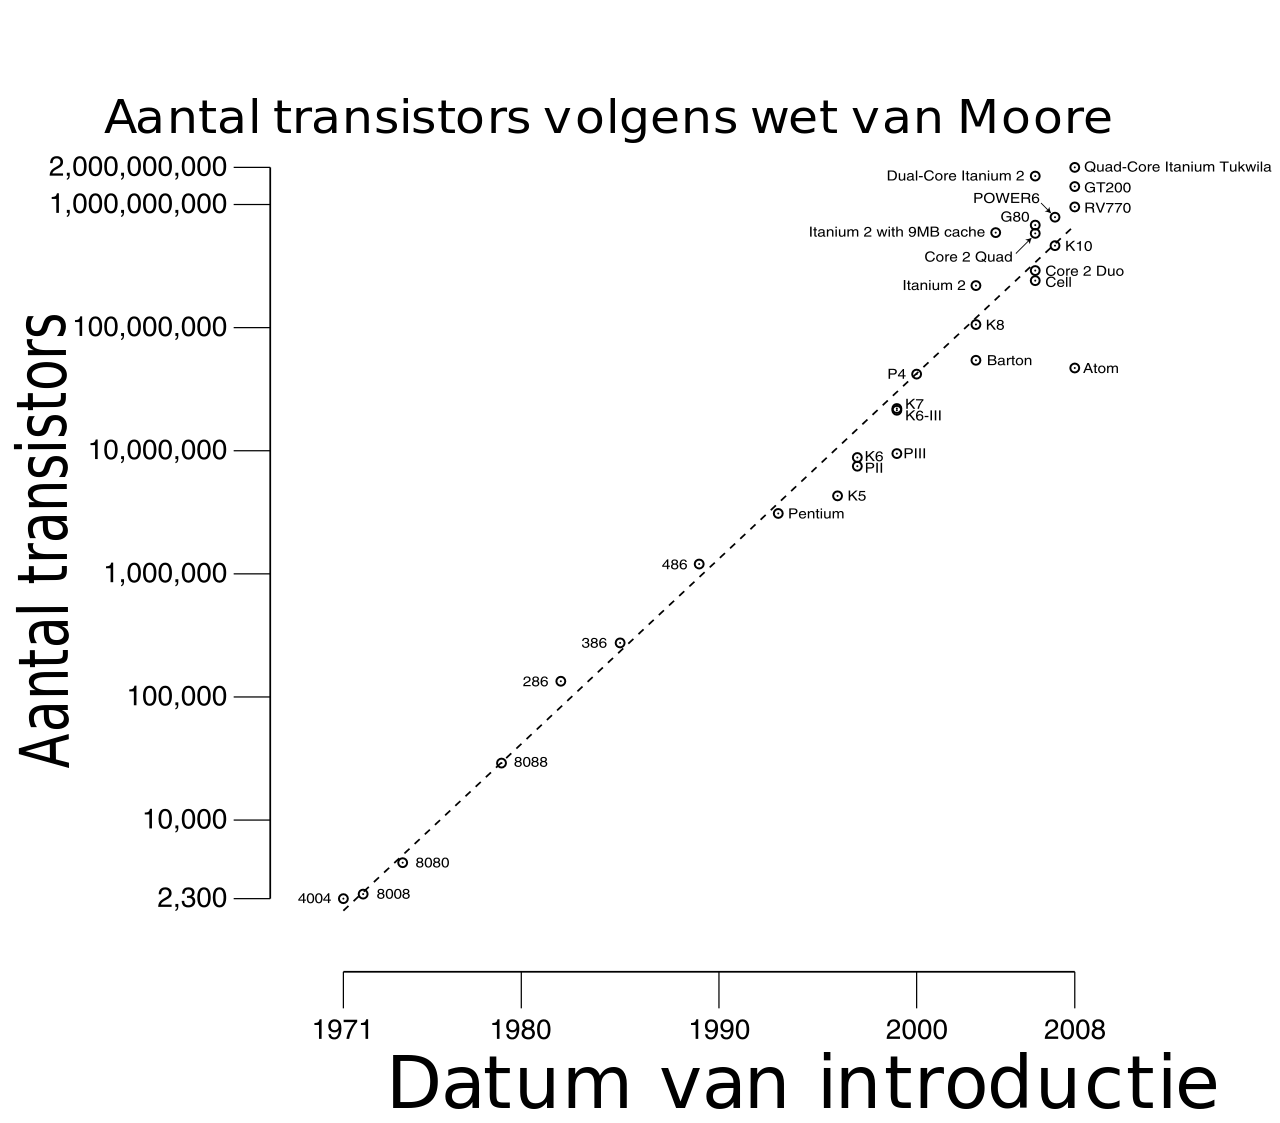
\includegraphics[width=\linewidth]{img/moore.png}
			\caption{De Wet van Moore.}
			\label{fig:moore}
		\end{figure}
		
		\subsection{Vereenvoudigde verificatie van betaling}
		Volgens \textcite{Nakamoto2008} is het mogelijk om betalingen te verifiëren zonder de hulp van een volledige netwerk-node, die ieder blok dat ooit gecreëerd werd kent. Om een transactie te verifiëren, moet een gebruiker enkel een kopie hebben van de headers van alle blokken uit de langste keten. Deze kunnen alleen verkregen worden door de netwerk-nodes te bevragen en op een gegeven moment te beslissen dat men de langste ketting heeft gevonden. Vervolgens moet van deze ketting de tak van de hash-boom die de transactie aan het blok linkt worden genomen.
	
		Met deze hash-tak kan de gebruiker weliswaar niet de transactie zelf controleren, maar er kan aan de hand van de positie van de transactie-hash wel gecontroleerd worden of de transactie al geaccepteerd is door de node en het netwerk.
		
		Op deze manier is verificatie gemakkelijk, op voorwaarde dat eerlijke nodes controle hebben over het netwerk. Nodes kunnen transacties altijd zelf verifiëren, maar de vereenvoudigde methode kan beetgenomen worden door aanvallers die meer dan de helft van het netwerk controleren. Een mogelijke strategie hiertegen zou zijn om de volledige keten te downloaden wanneer er een ongeldig blok binnenkomt. 
	\subsection{Combineren en splitsen van transacties}
	Opdat er geen aparte transactie voor iedere munt die van eigenaar wisselt zou gemaakt moeten worden, voorziet \textcite{Nakamoto2008} een systeem waarin transacties gecombineerd en gesplitst kunnen worden. Zo kan men bijvoorbeeld drie Bitcoins in één enkele transactie versturen, maar ook 0,5 Bitcoin als wisselgeld ontvangen.
	
	Om dit mogelijk te maken wordt er gewerkt met een systeem van inputs en outputs. Een transactie kan één of meerdere inputs hebben en één of twee outputs. De inputs staan voor de bron(nen) waar het geld vandaan komt, eender welke waarde in Bitcoin kan hier meegegeven worden. De outputs staan voor de ontvangende kant, de eerste is de waarde voor de ontvanger, de tweede output is optioneel en is voor het eventuele wisselgeld dat de verzender kan ontvangen.
	\subsection{Privacy}
	In het traditionele monetaire systeem ligt alle kennis over transacties bij de financiële instituties. De bank, als vertrouwde derde partij, kan gemakkelijk privacy creëren door de toegang tot informatie over een transactie te limiteren tot de betrokken partijen. 
	
	In het model dat we vanaf nu \textit{blockchain} zullen noemen, is deze methode onmogelijk door de noodzaak tot publiek aankondigen van transacties over het hele netwerk.  \textcite{Nakamoto2008} stelt echter dat privacy wel enigszins kan worden behouden door informatie op een andere plaats te beperken. Men stelt voor om de publieke sleutels, die Bitcoin-portefeuilles identificeren, anoniem te houden en er dus geen naam aan te koppelen. Hoewel iedereen op deze manier kan zien welke transacties er plaatsvinden, door de anonimiteit van zender en ontvanger wordt privacy grotendeels gegarandeerd.
	
	Om de privacy verder te verbeteren zou men ook kunnen opteren voor een systeem waarin iedere gebruiker per transactie een nieuwe sleutel krijgt, die uniek identificerend is. Bij transacties met meerdere inputs is er echter geen manier om te verbergen dat de inputs van een bepaalde eigenaar afkomstig zijn.
	\subsection{Nakamoto’s conclusie}
	In het paper presenteert men een nieuw systeem voor elektronische transacties. Men start vanuit munten die opgemaakt zijn uit digitale ondertekeningen. Vervolgens lost men het double-spending probleem op. Om dit te doen wordt er een peer-to-peer netwerk voorgesteld, dat gebruik maakt van zogenaamde proof-of-work om de historiek van gemaakte transacties op te slaan. 
	
	De implementatie maakt het computationeel onpraktisch om het systeem aan te vallen voor frauduleuze doeleinden. Het is immers een robuust netwerk met weinig complexe structuur waar anonimiteit en privacy grotendeels gerespecteerd blijven. ~\autocite{Nakamoto2008}
	
	Nodes binnen het netwerk werken allemaal tegelijk, doch zonder enige coördinatie of afhankelijkheid. Ze kunnen het netwerk verlaten en zich naar believen weer vervoegen. Nodes die zijn weggeweest moet enkel de volgende proof-of-work accepteren om weer helemaal mee te zijn met alles wat er is gebeurd. ~\autocite{Nakamoto2008}
	
	Er wordt gestemd op basis van CPU-kracht: het accepteren van een blok gebeurt door te beginnen werken aan de proof-of-work , het afwijzen ervan gebeurt door dat te weigeren. Op basis van dit consensus-mechanisme kunnen extra regels voor eender welke use-case worden toegevoegd. ~\autocite{Nakamoto2008}
	\newpage
\section{Ethereum en smart contracts}
\label{sec:ethereum-en-smart-contracts}
	\subsection*{Inleiding}
		In het tweede deel van dit hoofdstuk wordt een beeld geschetst van wat \textcite{Swan2015} blockchain 2.0 noemt, ofwel `Blockchain voorbij Bitcoin'. De concepten die in het vorige hoofdstuk werden besproken vormen de basis van de blockchain-technologie. De Bitcoin-blockchain staat intussen alweer een stuk verder en de Bitcoin is ook al lang niet meer de enige cryptomunt. De Bitcoin-blockchain is nu dus ook verre van de enige blockchain. Concreet wordt er in dit hoofdstuk dieper ingegaan op het concept  smart contracts, vervolgens wordt er ook een overzicht gegeven van Ethereum. Dit alles wordt uitgebreid besproken, omdat het van belang zal zijn eenmaal we blokchain-stemsystemen (zie \ref{sec:blockchain-gebaseerd-stemmen}) bespreken. \autocite{Buterin2014}
	\subsection{Noodzaak}
		\subsubsection{Wat  zijn smart contracts?}
			Smart contracts zijn een concept dat de blockchain-technologie een stap verder brengt. In \textcite{Swan2015} worden ze omschreven als gedecentraliseerde contracten, die niet langer een autoriteit (zoals een rechtbank) nodig hebben. Het zijn in feite digitale contractprogramma’s die zichzelf kunnen valideren en uitvoeren wanneer aan bepaalde voorwaarden is voldaan. Ook dit concept bestaat al sinds de jaren `90 ~\autocite{Szabo1996}. Bij het lezen van \textcite{Nakamoto2008} is het duidelijk dat er vanaf het prille begin van de Bitcoin een visie bestond om een dergelijke systeem te implementeren. Blockchain-technologie staat immers niet alleen de opslag van data toe, ook programma’s kunnen in de blockchain worden opgeslagen. Smart contracts vormen de basis van Blockchain 2.0 (de hedendaagse blockchain-technologie) en zowat iedere grote blockchain-speler probeert ze te implementeren~\autocite{Swan2015}.
		\subsubsection{Wat is Ethereum?}
			Ethereum (figuur \ref{fig:ethereum}) is een opensource-platform dat werd opgericht in 2015. Net zoals Bitcoin maakt het gebruik van een gedecentraliseerd netwerk. Het valideren van informatie gebeurt ook hier door zogenaamde miners, het verschil met Bitcoin is dat de miners worden beloond met de munteenheid `ether' in plaats van Bitcoin. Ethereum kan men niet zien als een zuivere variant op de Bitcoin of een andere vorm van cryptogeld, het is veel meer dan dat. Om te beginnen maken smart contracts  een groot deel uit van het Ethereum-ontwerp. \textcite{Swan2015} omschrijft Ethereum als een ``Turingcomplete Virtual Machine”, die zowel een platform als een programmeertaal genaamd \textit{Solidity} biedt voor het ontwikkelen en publiceren van gedistribueerde applicaties. Turingcompleetheid betekent in deze context dat het platform het vermogen heeft om eender welke digitale munt, protocol of blockchain te ondersteunen, iets wat bij de Bitcoin-blockchain niet het geval is \autocite{Swan2015}. Ethereum is momenteel\footnote{Op 1 juli 2019} na de Bitcoin de tweede grootste cryptomunt\footnote{Zie https://coinmarketcap.com/all/views/all/}. 
			
			\begin{figure}
				\centering
				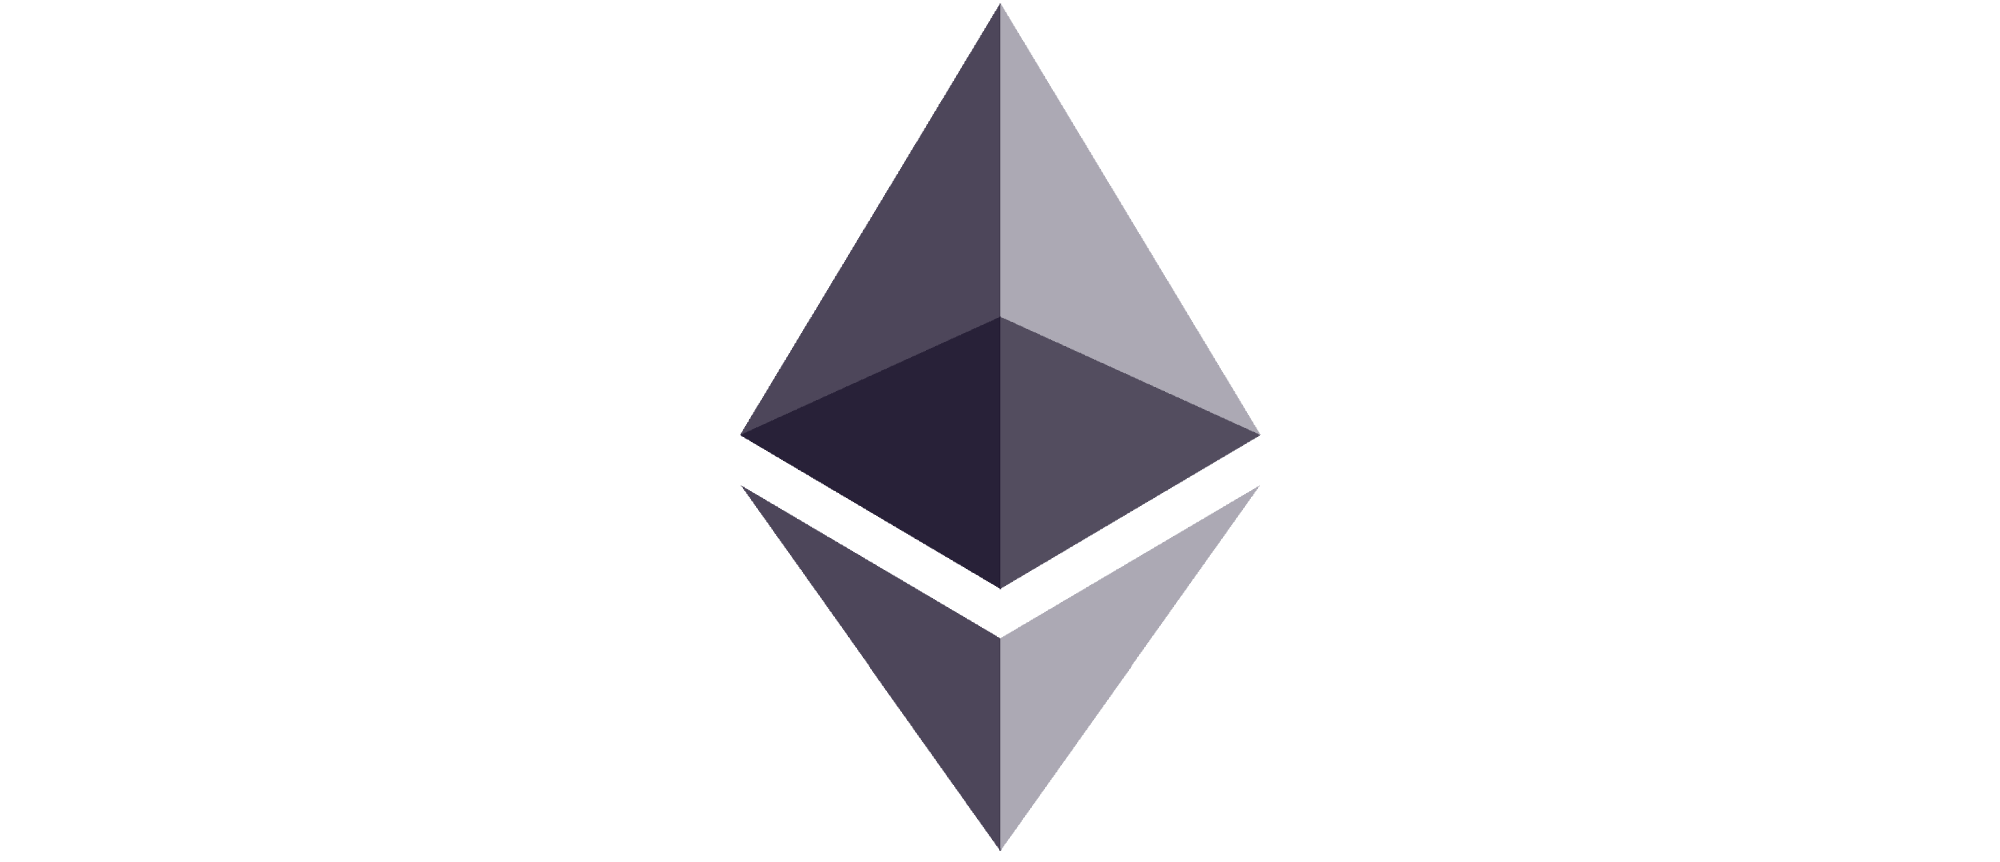
\includegraphics[width=\linewidth/2]{img/ethereum.png}
				\caption{Het Ethereum logo}
				\label{fig:ethereum}
			\end{figure}
			
			Ethereum is ontworpen met de volgende filosofie in gedachten ~\autocite{Buterin2014}\footnote{Zie https://github.com/ethereum/wiki/wiki/White-Paper\#ethereum}:
			\begin{itemize}
				\setlength\itemsep{1em}
				\item \textbf{Eenvoud}: 
				Een van de voornaamste doeleinden van Ethereum is om zo eenvoudig mogelijk te zijn, zelfs wanneer dit soms ten koste is van data-opslag of tijdsefficiëntie. Ethereum werd ontworpen met de bedoeling dat een gemiddeld ontwikkelaar, zonder diepgaande kennis van cryptografie, er applicaties op kan implementeren. De lage instapdrempel die de eenvoud van Ethereum creëert moet ertoe bijdragen dat het ongekende potentieel van cryptocurrencies en blockchain-technologie verder wordt uitgebouwd.
				\item \textbf{Universaliteit}: Ethereum doelt er op om Turingcompleet te zijn. Men wil  geen systeem aanbieden waar er gebruik kan worden gemaakt van bepaalde features, maar eerder een platform waarop ontwikkelaars zelf iedere mogelijke toepassing kunnen implementeren aan de hand van smart-contracts en transacties.
				\item \textbf{Modulariteit}: 
				Een ander belangrijk aspect in het ontwerp van Ethereum is modulariteit. De bedoeling is dat de verschillende onderdelen waaruit Ethereum is opgebouwd (zaken zoals Ethash, Patricia bomen en RLP) zo scheidbaar mogelijk worden gehouden. De verschillende bouwstenen worden als feature-complete bibliotheken gezien en kunnen ook buiten Ethereum worden gebruikt.
				\item \textbf{Agiliteit}: 
				Ethereum moet op een \textit{agile} manier worden ontwikkeld. Men moet heel flexibel kunnen zijn op het vlak van aanpassingen. Hoewel men heel voorzichtig is wanneer het aankomt op modificaties bij high-level constructies, heeft Ethereum ook het doel om nieuw-ontdekte mogelijkheden die verbetering brengen aan het systeem zo snel mogelijk te benutten.
				\item \textbf{Non-discriminatie en non-censuur}: 
				Tot slot zou Ethereum niet mogen aansturen op een bepaalde vorm van gebruik. De regulerende mechanismen in het protocol moeten op zodanige wijze ontwikkeld zijn, dat ze enkel de schade tegenhouden en geen specifieke ongewenste applicaties. Het voorbeeld van een oneindige lus wordt hier gegeven. Een applicatie die zo'n lus bevat is ongewenst, omdat ze middelen van het netwerk in beslag zal nemen en zo de verwerking van informatie zal vertragen. Toch wordt een dergelijke applicatie niet verboden door Ethereum. Het regulerende mechanisme dat een transactiekost per computationele stap garandeert zorgt er immers voor dat  het uitvoeren van een oneindige lus bijzonder nadelig wordt.
			\end{itemize}
	\subsection{Werking van Ethereum}
		De werking van het Ethereum-netwerk volgt op conceptueel niveau dezelfde lijnen als de eerder omschreven Bitcoin-blockchain~\autocite{Wood2017}. In dit segment wordt daarom vooral de focus gelegd op de verschillen tussen beide. 
		\subsubsection{Algemene verschillen tussen Bitcoin en Ethereum}
			In tegenstelling tot de (relatief) eenvoudige Bitcoin-transacties, bevatten de blokken die door het Ethereum-netwerk worden opgeslagen iets wat men zou kunnen omschrijven als een toestandsmachine, die bestaat uit een lijst van allerhande transacties. Waar de Bitcoin-blockchain in hoofdzaak ontworpen is om fiscale transacties mogelijk te maken, is de Ethereum-blockchain veel meer \textit{general-purpose}~\autocite{McCorry2017}. Om misbruik en spamming tegen te gaan en spoedige verwerking van transacties door nodes te stimuleren, is er aan iedere transactie een kleine kostprijs verbonden. Transactie- en uitvoeringskosten worden \textit{gas} genoemd en betaald in ether, het cryptogeld van Ethereum. De term gas is toepasselijk omdat men ether omschrijft als de brandstof waarop het Ethereum-netwerk draait ~\autocite{Buterin2014}\footnote{Zie https://github.com/ethereum/wiki/wiki/White-Paper\#messages-and-transactions}.
		\subsubsection{Ethereum-accounts}
		Binnen Ethereum is er sprake van twee soorten accounts: 
		\begin{itemize}
			\item \textbf{Accounts} van externe gebruikers, bestaand uit een publieke en private sleutel, dewelke een gebruiker in zijn bezit heeft.
			\item \textbf{Contract-accounts}, smart-contracts die bestaan uit code die enkel wordt uitgevoerd bij interactie met gebruikers.
		\end{itemize}	
		Zowel gebruikers als smart-contracts kunnen ether bezitten. ~\autocite{McCorry2017}
		\subsubsection{Ethereum-transacties}
			Naast beide accounttypes zijn ook transacties van significant belang voor de werking van Ethereum. De Ethereum-blockchain kan worden gezien als een geordende transactiestatus-machine~\autocite{McCorry2017}. Net als bij Bitcoin, zijn het de transacties die de kern van het systeem vormen. Ethereums transacties worden in een blockchain-structuur opgeslagen, wat een \textit{immutable} historiek van transacties oplevert en de huidige staat van het netwerk weergeeft. ~\autocite{Buterin2014}

		Een Ethereum-transactie bestaat uit de volgende velden ~\autocite{Buterin2014}:
		\begin{itemize}
			\item \textbf{From}: De ondertekening van het account dat de transactie autoriseert, dit kan alleen een gebruiker zijn.
			\item \textbf{To}: De ontvanger van de transactie, dit kan zowel een gebruiker als een contract zijn. 
			\item \textbf{Data}: Een optioneel veld. Hier kan code worden meegegeven voor de creatie of voor het uitvoeren van een functie op een smart contract. 
			\item \textbf{Gas Price}: De kost in ether die de verzender betaalt per computationele stap.
			\item \textbf{Start Gas}: Het maximum aantal computationele stappen dat mag worden uitgevoerd.
			\item \textbf{Amount}: Het bedrag in ether dat wordt overgemaakt van zender naar ontvanger.
		\end{itemize}	
		\subsubsection{Transacties tussen accounts}
		Transacties in Ethereum vinden plaats tussen twee gebruikers of tussen een gebruiker en een smart contract. Een transactie tussen een gebruiker en een smart contract kan één of meerdere nieuwe transacties vanuit het contract naar andere gebruikers doen ontstaan. ~\autocite{Buterin2014}
		
		Tenslotte kan een transactie van een gebruiker naar een smart contract ook transacties naar andere smart contracts triggeren, die dan op hun beurt hetzelfde doen en zo een complexe kettingreactie creëren. ~\autocite{Buterin2014}
		
		De combinatie van mogelijke transacties en het potentieel dat smart contracts bieden, zorgt voor een systeem waarop in theorie iedere toepassing mogelijk is. ~\autocite{Wood2017}
		\subsubsection{Proof-of-stake}
			Een ander belangrijk aspect waarin Ethereum sterk verschilt met de Bitcoin-blockchain, is de manier waarop transacties worden verwerkt. Ethereum-transacties worden anders verwerkt, in die zin dat het netwerk\footnote{Sinds 30/06/2019} een compleet andere mining-methode gebruikt. Sinds de Ethereum 2.0 update, is men namelijk overgeschakeld van \textit{proof-of-work mining} naar een algoritme dat \textit{proof-of-stake forging} genoemd wordt. Het is een alternatieve manier om aan `mining' te doen, die enkele significante voordelen biedt ten opzichte van proof-of-work. 
		
		De hoofdredenen om af te stappen van de klassieke mining-methode zijn:
		\begin{itemize}
			\item \textbf{Het netwerk is niet efficiënt}, miners zijn in directe competitie met elkaar, alle miners proberen gelijktijdig hetzelfde probleem op te lossen.
			\item \textbf{Het algoritme is niet efficiënt}, proof-of-work mining vergt dat nodes langdurig moeten zoeken op \textit{brute-force} wijze. 
			\item \textbf{Het vergt enorm veel energie}, omwille van de eerder genoemde gebreken.
		\end{itemize}
		 Proof-of-stake betekent een grote verbetering op deze vlakken. Het centrale idee bij proof-of-stake is dat alle nodes stakeholders zijn, die er belang bij hebben dat de transacties correct verlopen. Net zoals de miners worden de \textit{forgers} van proof-of-stake beloond voor hun werk via transactiekosten. Het grote verschil is echter dat forgers geen complex probleem moeten oplossen. Ze hoeven ook niet als eerste in iets te slagen om transacties te mogen verwerken. Iedere forger zet een zelfbepaalde monetaire waarde in als stake, de verhouding van deze waarde ten opzichte van de totale waarde aan stakes binnen het netwerk bepaalt het aandeel van de transacties dat door de forger mag verwerkt worden.
	\subsection{Conclusie}
		 Ethereum is een platform dat blockchain-technologie beschikbaar en toegankelijk maakt voor gewone ontwikkelaars. Een van Ethereums hoofddoelen is dan ook om \textit{multi-purpose} te zijn: het is bedoeld als een platform waarop iedere mogelijke toepassing geïmplementeerd kan worden. ~\autocite{Buterin2014}
		 
		 In deze sectie bespraken we de filosofie waarrond Ethereum ontworpen is. In het algemeen kan men stellen dat de focus vooral ligt op de functionaliteit en gebruiksvriendelijkheid naar ontwikkelaars toe. Voorbeelden hiervan zijn de keuzes op het vlak van \textit{modulariteit} en \textit{agiliteit}. ~\autocite{Buterin2014}
		 
		 Interacties met Ethereum gebeuren via smart contracts, in feite zijn het stukken code, kleine applicaties die op de blockchain draaien. Smart-contracts maken deel uit van de gedecentraliseerde structuur, daarom spreekt men ook wel van \textit{decentralized applications} of \textit{DApps}. ~\autocite{McCubin2019}
		 
		 Men probeert met Ethereum duidelijk een omgeving te creëren waarin er zoveel mogelijk vrijheid is op vlak van type implementatie, geen enkele applicatie wordt geweerd op basis van haar functie. Alleen applicaties die voor schade aan het netwerk zelf zorgen worden niet toegelaten, om de werking van de volledige blockchain intact te houden. ~\autocite{Buterin2014}
		 
		 Tenslotte bespraken we ook enkele nadelen aan de werking van huidige proof-of-work systemen en hoe Ethereum daar een oplossing voor biedt. Ethereums overstap van een proof-of-work systeem naar een proof-of-stake systeem is een significante beslissing die het blockchain-netwerk efficiënter dan ooit kan maken op vlak van verwerkingscapaciteit en energieconsumptie. Het vergroot de kansen dat blockchain als technologie ooit een industriestandaard kan worden. ~\autocite{Buterin2014}
		\newpage
\section{Blockchain-gebaseerd stemmen}
\label{sec:blockchain-gebaseerd-stemmen}
	\subsection*{Inleiding}
			In het derde en laatste deel van dit hoofdstuk wordt blockchain-gebaseerd stemmen besproken. Ten eerste wordt de noodzaak aangebracht, daarna worden bestaande implementaties besproken. De werking en achterliggende theorie worden als laatste besproken. Concreet behandelen we het \textit{Open Vote Network}, een stemprotocol dat  aan de hand van smart contracts en Ethereum wordt geïmplementeerd. We bespreken dit protocol omdat het een van de weinige blockchain-gebaseerde stemprotocollen is die volledig opensource is. Er zijn ongetwijfeld veel andere manieren om een blockchain-gebaseerd stemsysteem te realiseren. Hetgeen we hier bespreken is dus maar één voorbeeld, bedoeld ter illustratie.  In het vorige hoofdstuk bespraken we zowel Ethereum als smart contracts reeds uitvoerig, in dit hoofdstuk zal de focus daarom meer op het cryptografische aspect van het stemmen liggen. De werking van het stemprotocol wordt stap voor stap uitgelegd. De volledige natuur van de onderliggende cryptografie valt vaak buiten de scope van deze bachelorproef, bepaalde cryptografische technieken en wiskundige concepten worden daarom enkel vermeld en niet verder uitgewerkt. Tot slot wordt ook een selectie van bestaande implementaties besproken.
			Het concept blockchain-gebaseerd stemmen bevindt zich duidelijk nog in een vroeg stadium, men kan het zien als een onderdeel van wat \textcite{Swan2015} classificeert als blockchain 3.0 ofwel de blockchain-implementaties van de toekomst.
	\subsection{Noodzaak}
			\subsubsection{Democratie en stemmen}
			Democratie wordt gedefinieerd als: ``een systeem waarin het bestuur van een natie door de volledige bevolking gebeurt, of op zijn minst door de in aanmerking komende leden ervan''\footnote{ Definitie van democratie door Oxford Dictionairies, vertaald uit het Engels. Verkregen op 1 mei 2019 van https://en.oxforddictionaries.com/definition/democracy.}. In de meeste democratieën wordt het bestuur niet op directe wijze door de bevolking uitgeoefend, maar via verkozen vertegenwoordigers. Om een democratie te laten functioneren moeten er dus processen zijn om vertegenwoordigers aan te duiden.  Aan de basis van elke succesvolle democratie ligt daarom de voorwaarde dat men kan stemmen op een wijze die toegankelijk, veilig en correct is.~\autocite{Osgood2016}. 
			
			Klassieke verkiezingen gebeuren aan de hand van een stem op papier: men duidt de voorkeur aan op een stembiljet, vouwt het dicht en werpt dit vervolgens in een `zwarte doos' waarin alle stembiljetten ongeopend blijven tot ze worden geteld. Het tellen gebeurt handmatig: ambtenaren of burgers worden door een centraal stembureau opgeroepen om de lokale stemmen te tellen. De resultaten worden vervolgens doorgeven aan hogere niveaus tot er uiteindelijk een volledig resultaat bekend is\footnote{Omschrijving van hoe stemprocessen op papier doorgaans verlopen, lokale variaties zijn uiteraard mogelijk.}.
			
			\subsubsection{Elektronisch stemmen}
			Hoewel de papieren stem al eeuwen gebruikt wordt, zijn er toch een aantal problemen aan verbonden. In recente decennia heeft het zogenaamde elektronisch stemmen dan ook een enorme opkomst gekend. Ook in België, met name het Vlaamse Gewest, is dat het geval: in maar liefst de helft (157/300) van de Vlaamse gemeenten wordt vandaag gebruik gemaakt van stemcomputers (figuur \ref{fig:evote_vlaanderen}).
			
			\begin{figure}
				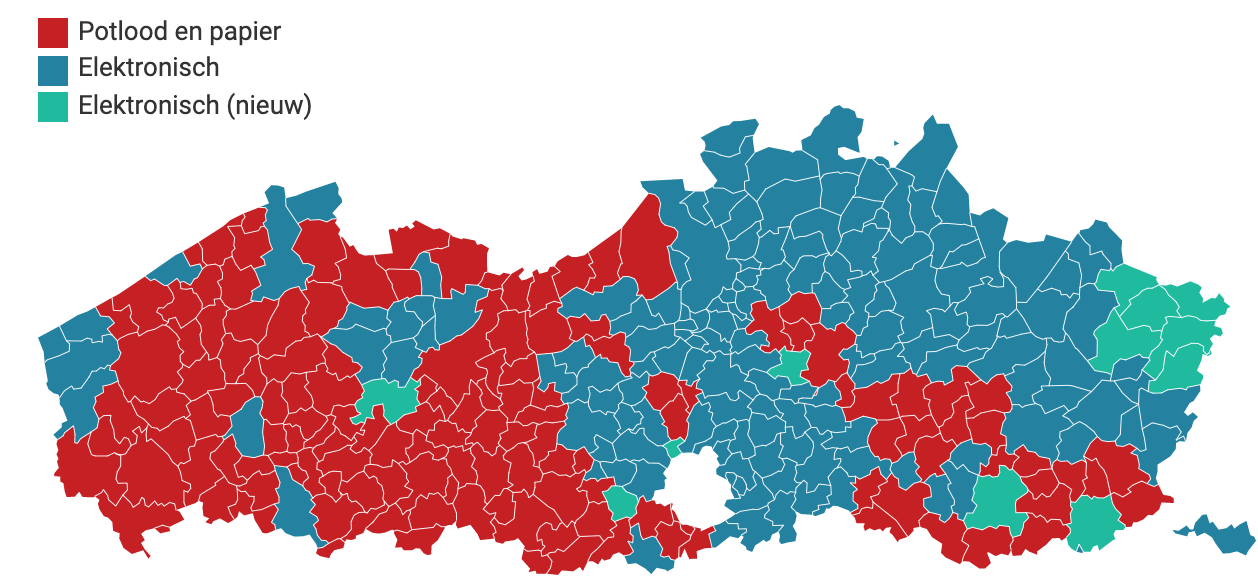
\includegraphics[width=\linewidth]{img/evote_vlaanderen.png}
				\caption{De helft van de Vlaamse gemeenten stemt digitaal (2018)}
				\label{fig:evote_vlaanderen}
			\end{figure}
			
			Volgens \textcite{Smartmatic2018}, leverancier van de stemcomputers in België en vele andere landen, biedt de elektronische stem een aantal aanzienlijke voordelen ten opzichte van de klassieke, papieren stem. Een van de voornaamste argumenten is dat de correctheid van de papieren stem in vraag kan worden gesteld, gezien het proces bijzonder gevoelig is voor menselijke fouten, al dan niet opzettelijk. Een ander argument is dat de papieren stem veel minder \textit{toegankelijk} en \textit{efficiënt} is. Elektronisch stemmen daarentegen, zou het stemproces voor vrijwel iedereen toegankelijk maken, ook personen met een lichamelijke of verstandelijke beperking zouden hiermee hun stem zelfstandig èn met behoud van het stemgeheim kunnen uitbrengen. Tenslotte is de elektronische stem volgens \textcite{Smartmatic2018} ook efficiënter (en dus economisch voordeliger) dan de papieren variant. Elektronisch stemmen is namelijk veel sneller, het stelt grote landen in staat de resultaten van hun verkiezingen in enkele uren te bereken, in plaats van enkele weken. ~\autocite{Smartmatic2018}
			
			\subsubsection{Problemen met elektronisch stemmen}
			Hoewel de genoemde argumenten voor elektronisch stemmen grond hebben, zijn er ook argumenten tegen het elektronisch stemmen te voeren. Uit het onderzoek \textcite{Norden2015} blijkt bijvoorbeeld dat een groot deel van de stemcomputers gebruikt voor verkiezingen in de VS sterk verouderd zijn. Naar schatting werden in 2015 in maar liefst 43 van de 50 staten stemcomputers gebruikt die minstens tien jaar oud waren, in 14 staten zouden er machines van meer dan 15 jaar oud zijn gebruikt. De leeftijd van de stemcomputers zorgde volgens \textcite{Norden2015}  voor problemen tijdens de congresverkiezingen van 2014, gaande van vastlopende en uitvallende machines met lange wachtrijen als gevolg, tot verloren en verkeerd geregistreerde stemmen (op een andere kandidaat) met incorrecte verkiezingsresultaten als gevolg.
			
			Verouderde software zorgt ervoor dat machines die gebruik maken van internetconnecties bijzonder kwetsbaar zijn. De beveiliging van zulke machines is niet meer adequaat volgens hedendaagse encryptiestandaarden. Externe partijen kunnen in theorie tijdens verkiezingen zonder veel moeite toegang krijgen tot de zulke stemcomputers. Verouderde hardware zorgt er dan weer voor dat reparatie- en onderhoudskosten voor oude stemmachines bijzonder hoog zijn~\autocite{Norden2015}.
			
			Ook in België en Nederland krijgt elektronisch stemmen vaak de wind van voren. Tijdens de Belgische federale verkiezingen van 2014 bleek bijvoorbeeld dat er bij 57 stemcomputers een probleem had plaatsgevonden, waardoor in totaal 2250 stemmen verloren gingen. In reactie daarop besliste Wallonië in 2015 voor een volledige terugkeer naar de papieren stem~\autocite{Maddens2018}.  In Nederland werden stemcomputers reeds in 1996 geïntroduceerd, maar ook hier zorgden toenemende problemen uiteindelijk in 2009 voor een volledige terugkeer naar potlood en papier ~\autocite{Schellevis2018}.
			
			\subsubsection{Blockchain-gebaseerd stemmen}
			Het is duidelijk dat er goede argumenten voor en tegen zowel papier als elektronisch stemmen gevoerd kunnen worden. Een blockchain-gebaseerd stemsysteem zou volgens proponenten van de technologie een nieuwe manier kunnen vormen om elektronisch stemmen te realiseren. Het zou veel van de huidige nadelen en problemen van elektronisch stemmen kunnen elimineren, en tegelijk ook de bestaande voordelen ten opzichte van stemmen op papier behouden. De gedistribueerde aard van blockchain zou er bovendien voor kunnen zorgen dat verkiezingen transparanter, veiliger en correcter dan ooit kunnen verlopen. 
			 
	\subsection{Bestaande implementaties}
			\subsubsection{Concrete toepassingen}
			Tot op heden zijn operationele toepassingen van blockchain-stemsystemen nog relatief zeldzaam.  Er dient wel  een onderscheid te worden gemaakt tussen de verschillende soorten toepassingen. Men kan  blockchain-technologie immers op diverse wijzen inzetten in de context van verkiezingen. In veel gevallen wordt een blockchain enkel ter ondersteuning van een groter stemsysteem gebruikt. Dit kan bijvoorbeeld zijn door blockchain als  een onveranderlijke opslagplaats te gebruiken voor de resultaten van een verkiezing. Een andere mogelijkheid is om blockchain-technologie als verificatie-tool te gebruiken  ~\autocite{Kshetri2018}. Er zijn echter ook implementaties die volledig blockchain-gebaseerd zijn. Voor dit onderzoek zijn deze implementaties natuurlijk het interessantste.
			
			In de volgende paragrafen worden vier recente cases besproken waarin blockchain-stemsystemen werden gebruikt ~\autocite{Kshetri2018}:
			\begin{enumerate}
				\item Parlementsverkiezingen in Sierra Leone
				\item De jaarlijkse algemene vergadering van het Estse technologiebedrijf LVH Groep
				\item Gemeenschapsprojecten in de Zuid-Koreaanse provincie Gyeonggi-do
				\item Het Active Citizen-programma van de stad Moskou
			\end{enumerate}
				
				\paragraph{Parlementsverkiezingen in Sierra Leone}
				In maart 2018 werd in Sierra Leone blockchain-technologie gebruikt om een kleine deelset van de resultaten van de nationale verkiezingen te controleren. Het systeem werd opgezet door het Zwitsers bedrijf Agora, dat aanwezig was als internationaal waarnemer van de verkiezingen. Agora creëerde veel oproer door miscommunicaties de wereld in te sturen, die deden lijken alsof de hele verkiezing op hun blockchain-systeem was gebeurd. In feite zorgde Agora's implementatie enkel voor het tellen en bewaren van resultaten op basis van een blockchain. Bovendien werd slechts een fractie van de populatie geobserveerd en de manier waarop dit gebeurde was erg foutgevoelig. Men verzamelde, onafhankelijk van de verkiezingen, via bevraging het stemgedrag van ruim 400,000 kiezers. Tijdens dit verzamelen werd de data live aan een blockchain-systeem gevoed. Het resultaat werd op gedistribueerde wijze berekend, ettelijke dagen voordat de klassieke telling was afgerond. De resultaten van Agora's telling kwamen echter niet overeen met die van de overheid. Dit voorbeeld, hoewel niet bepaald  inspirerend op vlak van correctheid en fouttolerantie, is toch opmerkelijk omdat het wel aantoont hoeveel sneller en efficiënter blockchain-systemen kunnen werken in vergelijking met klassieke manuele tellingen. ~\autocite{Kshetri2018}
				
				\paragraph{De jaarlijkse algemene vergadering van het Estse technologiebedrijf LVH Groep}
				Aandeelhouders van de Estse onderneming LVH Groep maken sinds 2015 gebruik van een kleinschalig online blockchain-gebaseerd stemsysteem ~\autocite{Kshetri2018}. LVH Groep is een financiële dienstenbedrijf dat zich gespecialiseerd heeft in blockchain-technologie, onder meer door het ontwikkelen van een Bitcoin-wallet \footnote{https://www.coindesk.com/lhv-bank-backs-wallet-app-built-on-Bitcoins-blockchain}. Doordat LVH groep een internationale onderneming is met kantoren in verscheidene landen, was het enorm kostelijk en tijdrovend om alle aandeelhouders op één plaats te verzamelen voor de jaarlijkse algemene vergadering. Er was  nood aan een veilig systeem om beslissingen over het internet te kunnen maken. Hiertoe werd, in samenwerking met onder andere de bedrijven NASDAQ en Chain ,een systeem geïmplementeerd op de Bitcoin-blockchain dat werkt op basis van smart contracts. Verificatie van de kiezers wordt gedaan door middel van het bestaande digitale identiteitssysteem in Estland \footnote{http://francescoolcelli.blogspot.com/2017/01/is-blockchain-answer-to-e-voting-nasdaq.html|}. Bijzonder aan deze implementatie is dat ze aantoont dat, ook zonder directe ondersteuning van het platform, er op blockchain zeer veilige en betrouwbare implementaties gemaakt kunnen worden. ~\autocite{Kshetri2018}
				
				\paragraph{Gemeenschapsprojecten in de Zuid-Koreaanse provincie Gyeonggi-do}
				In maart 2017 maakte het provinciebestuur van het Zuid-Koreaanse Gyeonggi-do gebruik van een blockchain-implementatie om burgers via directe verkiezingen te laten  bepalen welke gemeenschapsprojecten gefinancierd dienden te worden. Burgers konden zelf voorstellen doen en op suggesties van medeburgers stemmen. Het overkoepelende Ddabok Community Support Project zag maar liefst 9000 inwoners participeren. In totaal werden ongeveer 500  projecten geselecteerd voor subsidies. Het bijzondere aan deze implementatie was dat, hoewel georganiseerd vanuit de overheid, er geen enkele centrale autoriteit in het stemproces was betrokken. Het hele systeem werd ontwikkeld door Blocko, de grootste Zuid-Koreaanse blockchain-firma. ~\autocite{Kshetri2018}
				
				\paragraph{Het Active Citizen-programma van de stad Moskou}
				De stad Moskou kent sinds 2014 een programma genaamd `Active Citizen', waarin haar inwoners via zowel mobiele als online applicaties (zie figuur \ref{fig:active_citizen}) kunnen stemmen over allerhande maatregelen, gaande van de naam voor een nieuwe metrotrein tot de kleuren van zetels in een nieuw sportstadion. Het Active Citizen-programma telt meer dan 2 miljoen geregistreerde kiezers, er werden tot heden al meer dan 92 miljoen stemmen op uitgebracht. De laatste jaren is er echter steeds minder vertrouwen in de stad wanneer het op het tellen van de stemmen aankomt. Om de inwoners gerust te stellen en vertrouwen terug te winnen, werd daarom in 2017 een private versie van de Ethereum-blockchain aan de architectuur van het project toegevoegd. ~\autocite{Kshetri2018}
				
				\begin{figure}
					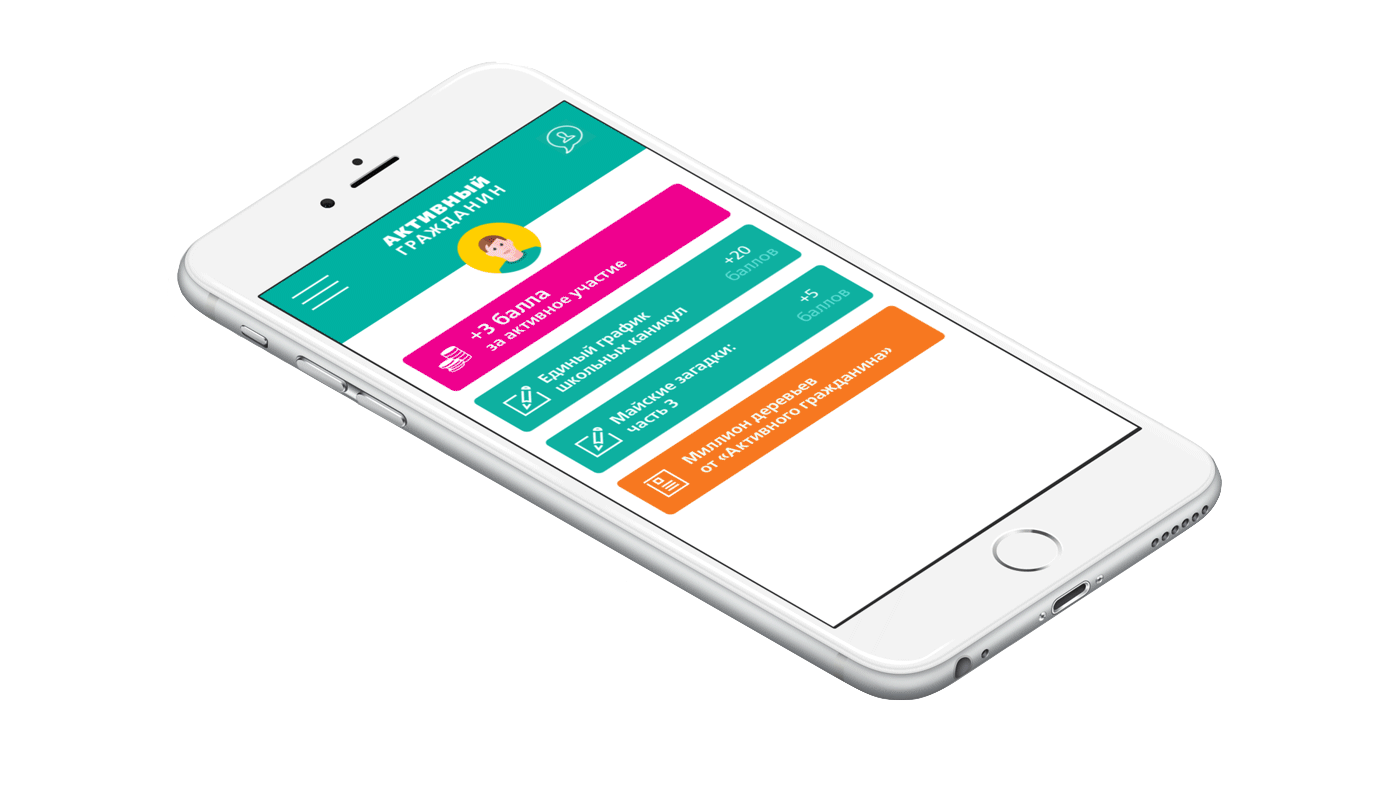
\includegraphics[width=\linewidth]{img/active_citizen.png}
					\caption{Het Active Citizen programma via een mobiele applicatie}
					\label{fig:active_citizen}
				\end{figure}
				
				Zoals vermeld gaat het om een private Ethereum-implementatie. Er wordt gewerkt aan de hand van smart contracts om de stemmen te registreren. Alle stemmen komen terecht in een  blockchain, het resultaat van alle verkiezingen is publiek toegankelijk. Ook de broncode voor de implementatie werd openbaar gemaakt op GitHub.
				
				De populairste onderwerpen zagen tussen de 137.000 en 220.000 participanten. Tijdens testen was de private Ethereum-implementatie in staat om tot 1000 transacties per minuut te verwerken. Het is niet duidelijk of de implementatie met  grotere volumes kiezers overweg zou kunnen. De schaalbaarheid is in deze context wel noodzakelijk: men wil een systeem bekomen dat toegankelijk is voor iedere bewoner, Moskou telt immers 12 miljoen inwoners. De kans is groot dat het huidige systeem overrompeld zou geraken en compleet verstoppen wanneer miljoenen kiezers hun stem gelijktijdig zouden uitbrengen.
				
				Op het vlak van security is schaalbaarheid dan weer geen probleem. De stadsadministratie liet het systeem testen door PwC, een internationaal accountants- en belastingadviseursbedrijf. De bevinding van PwC was dat er geen reden tot bezorgdheid is voor de veiligheid bij  300.000 of meer kiezers. 
				
				Al bij al levert dit voorbeeld toch een sterke case op voor blockchain-gebaseerd stemmen op grote schaal. Het toont aan dat men met voldoende middelen blockchain-stemprotocollen kan ontwikkelen die qua scope de klassieke board-room-voting systemen uit de literatuur vele malen overtreffen. 
			\subsubsection{Online diensten}
				\paragraph{Blockchain Voting Machine }
					Een van de grootste argumenten tegen blockchain-gebaseerd stemmen is dat het een verhoogd risico met zich meebrengt. De kans bestaat dat de nodes worden overgenomen of al overgenomen zijn. Voor een systeem dat werkt over het internet zou het gevaar van een nog grotere orde zijn. Blockchain Voting Machine is een algemeen concept dat hier een eenvoudig antwoord op biedt: men stelt voor om te werken met elektronische stemmachines zoals die vandaag al bestaan,  alleen zijn de machines aan een privaat blockchain-netwerk verbonden. 
				\paragraph{FollowMyVote}
					Het online stemplatform FollowMyVote hanteert de tegenovergestelde redenatie. Het uitgangspunt van dit opensource platform is net dat blockchain de ideale technologie is om verkiezingen niet alleen elektronisch maar ook online te laten verlopen. Online-verkiezingen zijn nodig volgens FollowMyVote, omdat het de kosten van verkiezingen enorm kan drukken en de opkomst van kiezers vele malen kan vergroten.  Niet alleen zwakkere groepen zoals bejaarden en individuen met een beperking, maar ook mensen in het buitenland kunnen meestemmen.  Op het vlak van identificatie stelt men voor om te werken met behulp van webcams en door de overheid uitgegeven identiteitsbewijzen. De resultaten van de verkiezingen worden in de blockchain opgeslagen en zijn publiek verifieerbaar. FollowMyVote stelt ook een reeks andere functionaliteiten voor, waaronder het in real-time volgen van verkiezingen en de mogelijkheid om de stem binnen de verkiezingstermijn aan te passen. 
				\paragraph{TIVI}
					TIVI hanteert heeft ongeveer dezelfde motivatie als FollowMyVote, maar op vlak van identificatie gaat men hier nog een stap verder. Men stelt voor om stemmen mogelijk te maken vanaf eender welk platform: laptop, mobiel of tablet. Verificatie kan volgens TIVI volledig via gezichtsherkenning gebeuren, men kan zich  identificeren door een selfie te nemen.
				\paragraph{Agora}
					Agora is een Zwitsers bedrijf dat een platform ontwikkelde voor blockchain-gebaseerde stemsystemen. Agora heeft een eigen custom blockchain-infrastructuur opgezet en bouwt middel tot grote verkiezingstoepassingen op maat voor haar klanten. Agora geldt momenteel als een van de grootste spelers in de sector.
					
	\subsection{Cryptografie en stemprotocollen}
		\subsubsection{Verschillende protocollen}
		\textcite{Kiayias2002} stelt voor om stemprotocollen \textit{self-tallying} te maken. Self-tallying ofwel zelftellend wordt hier gedefinieerd als volgt: iedere kiezer moet na het einde van een stemming zelf de stemmen kunnen tellen. Zelftellende stemprotocollen nemen de verantwoordelijk voor het tellen van stemmen weg van centrale autoriteiten en veranderen het in een open procedure, die iedere deelnemer of derde partij kan uitvoeren. De centrale autoriteit is dan niet langer nodig, iedereen kan resultaat van de stemming onafhankelijk bekomen. Men definieert ook twee andere eigenschappen waaraan een elektronisch stemprotocol moet voldoen.  \textit{Perfect Ballot Secrecy} ofwel volledige stembescherming, wordt gedefinieerd als een eigenschap die verzekert dat de privacy van de kiezer enkel en alleen ondermijnd kan worden wanneer alle andere kiezers tot dit doeleinde collaboreren. \textit{Dispute-freeness} (geschilloosheid), wordt dan weer gedefinieerd als een eigenschap die garandeert dat er geen twijfel kan zijn over de authenticiteit van de verkiezing. Deze eigenschap bestaat erin dat iedere participant,  voor zichzelf na afloop het correcte verloop van de procedure kan verifiëren.
			
		Volgens \textcite{McCorry2017}  hebben deze zelftellende protocollen echter zwaktepunten op het vlak van eerlijkheid. Ze staan toe dat kiezers die op een bepaald tijdstip hebben gestemd kunnen collaboreren om tussentijdse resultaten te berekenen voor datzelfde tijdstip. Verder kan de laatste persoon die zijn of haar stem moet uitbrengen het resultaat van de stemming berekenen voor hij of zij effectief gestemd heeft. Dit leidt volgens \textcite{McCorry2017} tot \textit{adaptive} en \textit{abortive issues}.  \textcite{McCorry2017} spreekt van een adaptive issue waar de stemkeuze van de laatste participant mogelijks beïnvloed kan worden door het zien van de stemresultaten alvorens zelf te stemmen. Er is volgens \textcite{McCorry2017}  ook sprake van een abortive issue omdat iedere participant de macht heeft om de hele stemming te annuleren. Een enkele participant kan zich immers volledig onthouden en zo alle andere kiezers verhinderen om het resultaat te berekenen. 
			
		\textcite{Kiayias2002} stelt dat het bovenstaande probleem makkelijk te corrigeren valt door middel van een extra stemronde. \textcite{McCorry2017} stelt echter dat daarvoor de volledige coöperatie van alle participanten nodig is, en dat deze op dat punt niet meer gegarandeerd is. Ook wordt er voorgesteld om de laatste stem steeds een lege stem van de organisator te laten zijn, maar ook hiertegen verzet \textcite{McCorry2017} zich, stellende dat dit in essentie een terugkeer is naar een systeem met centrale autoriteit.  \textcite{McCorry2017} stelt een protocol voor op basis van het werk van \textcite{Kiayias2002}, maar combineert als eerste het concept van self-tallying met een blockchain-implementatie. Het resulterend protocol noemt men het \textit{Open Vote Network Protocol} (OVNP).
		
		 \textcite{McCorry2017} maakt gebruik van Ethereum als ontwikkelingsplatform voor het OVNP. In sectie \ref{sec:ethereum-en-smart-contracts} bespraken we de verschillende voordelen die dit platform biedt reeds uitgebreid. Ook  stelt met BroncoVote een stemsysteem voor dat werkt via Ethereum. BroncoVote is blockchain-stemsysteem dat gebaseerd is op andere cryptografische methodes dan OVNP en bijgevolg sterk verschilt met de protocollen van \textcite{Kiayias2002} en \textcite{McCorry2017}. 
	
	\subsection{Het Open Vote Network Protocol}
	\label{sec:OVNP}
		\subsubsection*{Overzicht }
			Het Open Vote Network Protocol is een gedecentraliseerd protocol, ontworpen op basis van het self-tallying principe. De focus ligt hier op de bescherming van de privacy en robuustheid, niet op de schaalbaarheid. Self-tallying gebeurt immers niet op een wijze die bijzonder schaalbaar is. Het  OVNP ondersteunt bijgevolg enkel kleine verkiezingen met tientallen participanten, zaken zoals nationale verkiezingen zijn momenteel  zo goed als onmogelijk. Om de eenvoud te bewaren, wordt er gewerkt met het eenvoudigst mogelijke verkiezingspatroon, deelnemers hebben de keuze tussen twee opties, bijvoorbeeld een ja/neen-vraag.  \textcite{McCorry2017} verwijst naar het onderzoek van \textcite{Hao2009} voor zogenaamde multi-way verkiezingen ofwel verkiezingen met meerdere keuzeopties. 
			
			Het stemmen in dit protocol gebeurt in twee fasen: in de eerste fase laten alle kiezers zich registreren, in de tweede fase wordt de effectieve stem uitgebracht. Na afloop van de tweede fase kunnen de stemmen worden geteld.  De self-tallying eigenschap stelt iedere stakeholder die het protocol uitvoert ertoe instaat om zelf de stemmen te tellen. Merk op dat iedereen dit facet van het protocol kan uitvoeren, niet enkel de geregistreerde kiezers.
			 
			Het gedecentraliseerde karakter van dit protocol maakt het uiterst geschikt om op een blockchain te implementeren. \textcite{McCorry2017} is een van de eersten in de literatuur die deze stap maakt. De reden dat men specifiek voor de Ethereum-blockchain kiest wordt gemotiveerd als volgt.
			
			Andere blockhains zoals Bitcoin zouden ook kunnen worden gebruikt als publieke opslagplaats van verkiezingen, maar het verschil is dat het protocol zelf niet op de blockchain kan opgeslagen worden, het moet extern opgeslagen en gehandhaafd worden door de kiezers. \textcite{McCorry2017} stelt dat men via Ethereum gebruik kan maken van een smart-contract om  het protocol af te dwingen. Daarnaast kan Ethereum niet alleen als opslag fungeren, maar ook als geverifieerd netwerk waarover de participanten communiceren.
		\subsubsection*{Fase 0: setup }
			Het OVNP start vanuit een zogenaamde \textit{election administator}, deze organisator van de verkiezingen initialiseert het protocol door een verkiezing aan te maken en de in aanmerking komende kiezers in te stellen. Dit gebeurt door de kiezers aan de white-list van het smart contract toe te voegen. De kiezers worden in dit stadium enkel geïdentificeerd aan de hand van hun Ethereum-account. De organisator is meestal degene die Ethereum verwittigt om over te schakelen naar de eerste fase.
		\subsubsection*{Fase 1: registratie }
			De administrator stelt het onderwerp van de verkiezing in, alsook de beschikbare opties waarvoor gestemd kan worden. Vervolgens wordt Ethereum opnieuw verwittigd, ditmaal om over te gaan naar de registratie van de participanten. Om te registreren voor de verkiezing, moeten alle kiezers vooraf een stemsleutel berekenen. Deze sleutel zal worden gebruikt ter identificatie van de kiezers. Het berekenen van de stemsleutel en het verdere verloop (samengevat in figuur \ref{fig:ovnp}) gaat als volgt: 
			
			Alle \textbf{\textit{n}} kiezers moeten het eens zijn over het paar \textbf{\textit{(G,g)}} waarbij \textbf{\textit{G}} een eindige cyclische groep van hoofdorde \textbf{\textit{q}} voorstelt waarop het Diffie-Hellman (DDH) probleem niet van toepassing is, en \textbf{\textit{g}} een generator in \textbf{\textit{G}}. De lijst van in aanmerking komende kiezers, hier ook participanten \textbf{\textit{(P$_{1}$, P$_{2}$, … , P${n}$)}} genoemd, wordt vastgelegd. Elke participant \textbf{\textit{P$_{i}$}} kiest een unieke random-waarde (\ref{formula0}).
			
			\begin{ceqn}
				\begin{align}
				x_{i} \in^{R} Z_{q}\label{formula0}\
				\end{align}
			\end{ceqn}	
			
			 De waarde \textbf{\textit{x$_{i}$}} wordt gebruikt als private stemsleutel. Iedere kiezer vormt zijn of haar publieke stemsleutel door \textbf{\textit{g$^{x_{i}}$}} te berekenen. Gezien \textbf{\textit{g}} een generator is van \textbf{\textit{G}}, valt niet te achterhalen aan de hand van \textbf{\textit{g$^{x_{i}}$}} wat de eigenlijke waarde van \textbf{\textit{x$_{i}$}} is. Het Ethereum-netwerk heeft met andere woorden geen kennis van \textbf{\textit{x$_{i}$}}. Om de participant \textbf{\textit{P$_{i}$}} te kunnen identificeren in het netwerk volstaat de publieke sleutel echter niet, er is ook een bewijs van de private sleutel \textbf{\textit{x$_{i}$}} nodig. Tot dat doeleinde wordt een Zero Knowledge Proof gebruikt. Met \textbf{\textit{ZKP(x$_{i}$)}} levert de participant \textbf{\textit{P$_{i}$}}  het bewijs aan het netwerk dat de \textbf{\textit{x$_{i}$}}  in \textbf{\textit{g$^{x_{i}}$}} gekend is door \textbf{\textit{P$_{i}$}}. Zonder de waarde voor \textbf{\textit{x$_{i}$}}  effectief bekend te maken, wordt op die manier bewezen dat \textbf{\textit{P$_{i}$}} de eigenaar van de publieke sleutel \textbf{\textit{g$^{x_{i}}$}} is.
			
			Registratie gebeurt door iedere kiezer \textbf{\textit{P$_{i}$}} te laten broadcasten naar het netwerk. De broadcast bestaat uit \textbf{\textit{g$^{x_{i}}$}}  en \textbf{\textit{ZKP(x$_{i}$)}}. Daarnaast wordt er ook een constante waarde in ether uit de portefeuille van de kiezer aan de broadcast toegevoegd. Het gaat hier om de som van de transactiekosten en een waarborg die de kiezer terugkrijgt. Het instellen van de waarborg gebeurt omdat blockchain-filosofie dicteert dat het verbinden aan een potentiële kost participanten zal stimuleren om oprecht te handelen. In dit geval geeft men de waarborg terug zodra hun stem is uitgebracht. 
			
			Nadat een kiezer \textbf{\textit{P$_{i}$}}  naar Ethereum heeft gebroadcast, zal het netwerk zijn broadcast verwerken. Het bewijs in de vorm van de \textbf{\textit{ZKP(x$_{i}$)}} wordt gecontroleerd, de waarborg opgeslagen en tot slot wordt de stemsleutel \textbf{\textit{g$^{x_{i}}$}} gebruikt om een nieuwe sleutel te berekenen, waarmee de kiezer \textbf{\textit{P$_{i}$}} een stem zal kunnen uitbrengen over het ingestelde onderwerp. Deze nieuwe sleutel noemt men de gereconstrueerde sleutel \textbf{\textit{g$^{y_{i}}$}}, ofwel \textbf{\textit{Y$_{i}$}} en wordt berekend als volgt: 
			\begin{ceqn}
				\begin{align}
					Y_{i} = \prod_{j=1}^{i-1}g^{x_{j}}  / \prod_{j=i+1}^{n}g^{x_{j}} \label{formula1}\
				\end{align}
			\end{ceqn}
			
			\eqref{formula1} \textit{Om de gereconstrueerde sleutel g$^{y_{i}}$ te berekenen van kiezer \textbf{P$_{i}$} worden de publieke stemsleutels van alle andere kiezers \textbf{P$_{j}$} gebruikt. Het product van de publieke sleutels van al de andere kiezers \textbf{P$_{j}$} waar j < i wordt gedeeld door het product van alle publieke sleutels van alle andere kiezers \textbf{P$_{j}$} waar  j > i.}
			
		\subsubsection*{Fase 2: stemmen}
			Eenmaal het netwerk signaal ontvangt dat er gestemd kan worden, kunnen de kiezers een beslissing maken en vervolgens hun stem broadcasten. Deze broadcast bestaat uit twee zaken: de geëncrypteerde stem en een nieuwe Zero Knowledge Proof, die bewijst dat de stem ofwel 0 of 1 is. De encryptie die gebruikt wordt voor de stem vormt het cryptografische hart van dit protocol. 
			
			De stem wordt geëncrypteerd volgens het Elgamal-cryptosysteem en wordt in de vorm  \textbf{\textit{g$^{x_{i}y_{i}}$g$^{v_{i}}$}} aan het netwerk doorgegeven,  waarbij  \textbf{\textit{g$^{x_{i}y_{i}}$}} het product is van de publieke stemsleutel en de gereconstrueerde sleutel, \textbf{\textit{v$_{i}$}} de eigenlijke stem is in de vorm van een 1 of een 0 en \textbf{\textit{g$^{v_{i}}$}} de factor waarmee het product van de sleutels vermenigvuldigt wordt, zijnde \textbf{\textit{g}} ofwel 1. 
			
			Eenmaal \textbf{\textit{P$_{i}$}} een stem broadcast, wordt aan de hand van de \textbf{\textit{ZKP(v$_{i}$)}} geverifieerd of de stem in een correcte format is (0 of 1). Is dit het geval, dan wordt de Elgamal-geëncrypteerde stem opgeslagen in de Ethereum-blockchain en wordt de waarborg aan \textbf{\textit{P$_{i}$}} geretourneerd.
			
			Wanneer alle  \textbf{\textit{n}} stemmen ontvangen en geverifieerd zijn, krijgt iedereen er toegang toe. De identiteit van de kiezer noch de betekenis is door de encryptie af te leiden uit een particuliere stem. Alleen het resultaat kan nog bekomen worden uit de nu persistente geëncrypteerde stemmen.
			
			Het resultaat van de verkiezing bekomt men door het product van alle geëncrypteerde stemmen te nemen \eqref{formula2}: 	
			\begin{ceqn}
				\begin{align}
				\prod_{i=1}^{n}g^{x_{i}y_{i}}g^{v_{i}} \label{formula2}\
				\end{align}
			\end{ceqn}	
			De aard van de encryptie is zodanig dat alle random factoren geëlimineerd worden \eqref{formula3}, zodat :	
			\begin{ceqn}
				\begin{align}
				\prod_{i=1}^{n}g^{x_{i}y_{i}} = 1 \label{formula3}\
				\end{align}
			\end{ceqn}
			Dit resulteert in:
			\begin{ceqn}
				\begin{align}
				g^{\sum_{i=1}^{n}v_{i}} \label{formula4}\
				\end{align}
			\end{ceqn}
			Waarbij \textbf{\textit{$\sum_{i=1}^{n}v_{i}$}} in \eqref{formula4} het aantal stemmen voor waarde 1 representeert. Het aantal ja-stemmen kan echter niet rechtstreeks worden afgeleid, \textbf{\textit{g}}  wegwerken impliceert een discreet logaritme. Gezien de rechterhelft van de vergelijking bekend is en \textbf{\textit{i}} gelimiteerd is tot het aantal participanten \textbf{\textit{n}}, is het vrij zeker dat het hier om een kleine waarde gaat. Deze waarde kan gemakkelijk gevonden worden door middel van \textit{brute-force} zoeken. Eenmaal het aantal ja-stemmen gevonden is, wordt het vinden van de neen-stemmen triviaal.
			
			Merk op dat het bij self-tallying stemprotocollen noodzakelijk is dat iedere kiezer die in fase 1 een stemsleutel broadcastte, ook een geëncrypteerde stem uitstuurt in fase 2. Zo niet kunnen de resultaten van de stemming niet worden berekend. Er is hier dus nog steeds sprake van een \textit{abortive issue}.
			
			Ook is er het feit dat bij self-tallying stemprotocollen de allerlaatste kiezer mogelijks de stemmen kan tellen alvorens zelf te kiezen. Door een 0-stem te simuleren, kan deze kiezer het resultaat van de verkiezingen berekenen voordat alle anderen dit kunnen. De kiezer kan dus potentieel zijn of haar stem nog veranderen op basis van het voorlopige resultaat van de verkiezing. In de meeste gevallen is dit natuurlijk geen wenselijke situatie. De oplossingen die voor dit probleem in de literatuur worden voorgesteld zijn volgens \textcite{McCorry2017} echter ook sub-optimaal. 
			
			\textcite{McCorry2017} stelt voor om een fase toe te voegen tussen de fases 1 en 2. In deze tussenfase wordt de stem van de kiezer opgeslagen voor bekendmaking aan het netwerk. Eenmaal opgeslagen kan de stem niet meer worden veranderd. De volgende fase bestaat er dan in de stem aan het netwerk bekend te maken. 

			\begin{figure}
				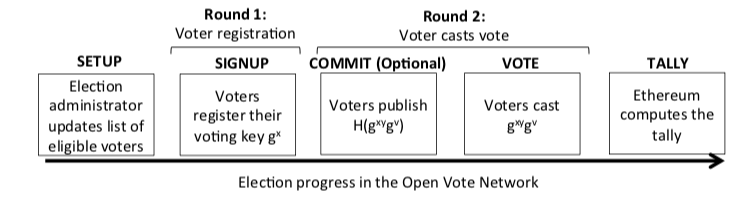
\includegraphics[width=\linewidth]{img/ovnp.png}
				\caption{Het Open Vote Network Protocol samengevat}
				\label{fig:ovnp}
			\end{figure} 
	
	\newpage
	\subsection{Privacy en transparantie}
		Typische elektronische stemprotocollen beschermen de privacy van kiezers door gebruik te maken van een centrale autoriteit. Om veiligheidsredenen is de autoriteit vaak verdeeld over verschillende tellingsautoriteiten. Een voorbeeld hiervan vinden we terug bij het stemsysteem van Helios\footnote{Zie https://github.com/benadida/helios-server}. Elektronische stemmen worden hier door meerdere tellingsautoriteiten behandeld. In combinatie met cryptografie reduceert men het risico op aantasting van de gebruikersprivacy aanzienlijk ~\autocite{Adida2008}. 
	
		Los van dit gegeven staat echter het feit dat een dergelijk systeem gebaseerd is op het vertrouwen van de kiezers. De mogelijkheid bestaat nog steeds dat alle tellingsautoriteiten van kwade wil zijn of dat ze simpelweg overrompeld worden door aanvallers. In zo’n situatie kan de privacy van de gebruikers alsnog geschonden worden. ~\autocite{McCorry2017}
		
		In essentie gaat het hier om een probleem op het vlak van transparantie. De gebruiker van het systeem heeft immers weinig tot geen middelen om zichzelf ervan te verzekeren dat het hele proces correct verloopt. ~\autocite{McCorry2017}
		
		We bespraken verschillende manieren waarop blockchain-technologie kan aangewend worden in elektronische stemsystemen. De verschillende wijzen die we bespraken kennen enkele noemenswaardige verschillen op het vlak van privacy. Het Open Vote Network dat voorgesteld werd door \textcite{McCorry2017}, vormt een van de meest robuuste structuren die de privacy van gebruikers garanderen. Volledige anonimiteit, zoals men die heeft bij het werpen van een papieren stem in de stembus, is niet mogelijk op blockchain. Op basis van cryptografie slaagt \textcite{McCorry2017} er wel in om het vinden van andermans identiteit praktisch onmogelijk te maken. Merk op dat  de term identiteit hier niet verwijst naar de persoonlijke gegevens van de gebruiker, maar wel naar het Ethereum-account.
		
		Ook  de andere systemen die we hebben besproken: Agora, FollowMyVote, enz. lijken op het eerste gezicht relatief goed te scoren op het vlak van privacy. Toch is er bij veel van de besproken voorbeelden een fundamenteel probleem op het vlak van centralisatie, aldus \textcite{McCorry2017}. De meeste voorgestelde oplossingen zijn nog steeds, in variërende mate, afhankelijk van een centrale autoriteit. Men zou het argument kunnen voeren dat bijvoorbeeld een bedrijf zoals FollowMyVote, hoewel het hele stemproces op de blockchain gebeurt, op een bepaalde manier zelf een centrale autoriteit wordt wanneer men van hun diensten gebruik maakt. Blockchain-gebaseerde stemsystemen waarvan de codebasis niet opensource is, vergen daarenboven op een bepaalde manier ook weer het vertrouwen van de gebruiker. Wanneer stemsystemen ook toegang krijgen tot gevoelige informatie zoals elektronische identiteitsgegevens of zelfs biometrische data voor gezichtsherkenning - zoals het bedrijf TIVI voorstelt -, dan speelt dit vertrouwen een rol die zodanig cruciaal is dat er eigenlijk sprake is van een centrale autoriteit.
	\subsection{Fouttolerantie, veiligheid en correctheid}
	
	Naast privacy en transparantie zijn ook fouttolerantie, veiligheid en correctheid van centraal belang in de context van stemprotocollen. Deze drie zaken zijn inherent met elkaar verbonden, er is zelfs sprake van zekere overlapping. We definiëren kort de bovenstaande termen voordat we bekijken hoe ze van toepassing zijn op blockchain-gebaseerde stemsystemen. \textit{Fouttolerantie} gaat in de eerste plaats over de robuustheid van het systeem: het is de mate waarin het systeem bestand is tegen allerhande fouten die zich kunnen voordoen. Een belangrijke distinctie is dat we het hier enkel over onopzettelijke fouten hebben. De mate waarin opzettelijke fouten en andere malafide acties een impact hebben op het systeem wordt gedefinieerd als de \textit{veiligheid}. Tenslotte definiëren we \textit{correctheid} als de mate waarin het berekende resultaat overeenkomt met de werkelijkheid en dit onder invloed van factoren zoals fouttolerantie en veiligheid.
	
	Op het vlak van fouttolerantie zijn er een paar inherente problemen met het OVNP dat \textcite{McCorry2017} voorstelt. De voornaamste problemen zijn zogenaamde \textit{abortive issues}, die te maken hebben met het missen van deadlines. Zoals vermeld wordt er in het OVNP gewerkt met verschilleden fases, alle kiezers worden steeds verondersteld om binnen deze fases bepaalde acties te ondernemen. Een kiezer die per ongeluk zo een deadline mist, bijvoorbeeld door het uitvallen van de netwerk-connectie, verliest niet alleen zijn voorafbetaalde waarborg, maar ondermijnt ook de volledige verkiezing. De cryptografie van het systeem vereist immers dat iedere geregistreerde kiezer een stem uitbrengt vooraleer de resultaten kunnen berekend worden. Ook op het vlak van veiligheid vormt dit een probleem, het betekent dat iedere participant voor de prijs van de waarborg de verkiezing kan boycotten. Tenslotte zal dit zich ook laten gelden op het vlak van schaalbaarheid en scope. 
	
	De andere kant van de medaille is hier dat het OVNP wel zeer goed scoort op het vlak van \textit{correctheid}: het is moeilijk om het resultaat op frauduleuze wijze te beïnvloeden. De enige manier waarop dit kan gebeuren is bij overname van het Ethereum-account van een gebruiker of bij overname van meer dan 50\% van het betreffende Ethereum-netwerk (er zijn verschillende Ethereum-netwerken). Beide situaties worden door \textcite{McCorry2017} als onwaarschijnlijk geacht, er wordt dus geen rekening mee gehouden. Voor de eerste situatie is het argument van \textcite{McCorry2017} dat het de verantwoordelijkheid van de gebruiker is om zichzelf en zijn Ethereum-account (portefeuille) te beschermen, voor de tweede situatie is het argument dat het zeer onwaarschijnlijk is dat een aanvaller er in slaagt om 51\% van de nodes over te nemen en zo de Ethereum-blockchain te vervalsen ~\autocite{McCorry2017}.
	
	 Het OVNP en andere blockchain-gebaseerde stemsystemen die we niet hebben besproken, zoals BroncoVote voorgesteld door \textcite{Dagher2018}, zijn niet zonder problemen wanneer het op fouttolerantie en veiligheid aankomt. De waarheid gebiedt echter om te zeggen dat dit voor geen enkel elektronisch systeem het geval is. Zelfs bij de elektronische stemmachines die in veel landen voor verkiezingen worden ingezet is er kans op een veelvoud van problemen, zo blijkt uit het \textcite{Norden2015} onderzoek. Internet-gebaseerd stemmen lijkt op het eerste zicht een goede oplossing te zijn, maar in feite vervangt het de bestaande problemen alleen maar door nieuwe, met grotere risico's. Veel experten hebben voorlopig nog grote bedenkingen bij online-stemmen ~\autocite{Norden2015}. 
	 
	 Een van de grootste bezorgdheden is dat het online-brengen van een stemsysteem de veiligheid van de verkiezing kan compromitteren, een online-systeem kan namelijk door om het even welke persoon of instantie worden aangevallen ~\autocite{Norden2015}. Vooral voor verkiezingen op nationaal of ander electoraal niveau vormt dit een serieus probleem. Recente gebeurtenissen hebben aangetoond dat dergelijke verkiezingen wel degelijk het doelwit van grote georganiseerde instanties, of zelfs volledige `vijandige' naties kunnen zijn. Als voorbeeld geven we hier de Amerikaanse presidentsverkiezingen van 2016, waar volgens het \textcite{Mueller2019} onderzoek Russische instanties op verschillende manieren het resultaat zouden hebben beïnvloed.
	 
	 In dit licht lijken blockchain-gebaseerde stemsystemen nog niet zo slecht, althans qua fouttolerantie, veiligheid en correctheid. Toch staan veel experts (zowel van blockchain-technologie als van stemsystemen) hier sceptisch tegenover. Het is duidelijk dat er nog veel problemen zijn die tot op heden de ingebruikname van blockchain-gebaseerde stemsystemen bemoeilijken. Bij de huidige stemsystemen blijken er ook heel wat problemen te zijn, soms zelfs in grotere mate. Er dient hier ook een distinctie gemaakt te worden tussen blockchain-gebaseerd stemmen en online stemmen. Hoewel veel van de huidige blockchain-implementaties - waaronder het OVNP - online implementaties zijn, is er geen verder verband tussenbeide. Implementaties binnen het concept Blockchain Voting Machine tonen aan dat blockchain-gebaseerd stemmen evengoed offline kan gebeuren, zonder internetverbinding. Veel problemen die online blockchain-gebaseerde implementaties hebben op het vlak van veiligheid, zijn eerder aan  het online aspect te wijten dan aan het blockchain aspect.
	
	\subsection{Schaalbaarheid en scope}
	We bespreken de schaalbaarheid en scope van blockchain-gebaseerde stemsystemen. Schaalbaarheid en scope kunnen makkelijk als synoniemen gezien worden, maar in deze context hechten we er verschillende betekenissen aan. Schaalbaarheid definiëren we als de mate waarin een stemsysteem kan groeien, dat wil zeggen de maximale hoeveelheid kiezers die het systeem kan ondersteunen. De scope definiëren we de dan weer als de context en het belang van de verkiezing. Bepaalde verkiezingen zijn immers van groter belang dan andere. Het verschil tussen schaal en scope is in veel gevallen wel subtiel, vaak is er een verband tussen de grote orde van een verkiezing en het belang ervan.
	
	De blockchain-gebaseerde stemsystemen die we tot nu toe hebben besproken, variëren in grote mate op het vlak van schaalbaarheid en scope. Een belangrijk onderscheid is het verschil tussen de systemen uit de praktijk en deze uit de literatuur. Praktijkvoorbeelden zoals het  \textit{`Active Citizens Project'} van Moskou ondersteunen tot 220.000 participanten, terwijl voorbeelden uit de literatuur zoals het  \textit{`Open Vote Network protocol'} en  \textit{`BroncoVote'} slechts een 30-tal participanten ondersteunen. Een mogelijke verklaring voor dit gegeven is dat de voorbeelden uit de literatuur simpelweg niet over dezelfde middelen beschikken als bijvoorbeeld het \textit{`Active Citizens Project'}. Een andere, zeer waarschijnlijke verklaring die hier ook bij aansluit, is dat het beschikken over een privaat blockchain netwerk, speciaal ontworpen voor verkiezingen, voor een groot verschil zorgt op het vlak van schaalbaarheid .
	
	 Zowel \textcite{McCorry2017} als \textcite{Dagher2018} benoemen Ethereums gebrek aan ondersteuning voor cryptografie als één van de primaire obstakels voor hun respectievelijke implementaties. Doordat er geen ingebouwde ondersteuning is vanuit \textit{Solidity}, moet men gebruik maken van externe bibliotheken. Dit resulteert in code die te omvangrijk is om in één smart contract op te slaan. Vandaar dat  \textcite{McCorry2017} en \textcite{Dagher2018} beiden met een stem- en cryptografiecontract werken. Cryptografische berekeningen zijn bovendien erg duur om uit te voeren in Ethereum, met als gevolg dat de verwerking van stemmen ook bijzonder langzaam gaat~\autocite{Dagher2018}.
	 
	 Op het vlak van schaalbaarheid lijkt er dus wel potentieel te zijn, maar voorlopig blijft dit niet het geval: de meeste blockchains kennen immers een inherent-slechte schaalbaarheid~\autocite{Blenkinsop2018}. Het fundamentele probleem is de grootte van ieder blok. Zowel de Bitcoin als de Ethereum-blockchain hebben blokken die steeds van dezelfde grote zijn, terwijl het aantal gebruikers en transacties toeneemt. Dit vormt een probleem, gezien de grootte van ieder blok rechtstreeks is verbonden aan het aantal transacties dat per tijdseenheid kan verwerkt worden. De Bitcoin-blockchain behandelt drie tot vier transacties per seconde, de Ethereum-blockchain doet er maar liefst 15. Dit betekent een beperking op het vlak van schaalbaarheid en scope. Stemprotocollen zoals het OVNP op Ethereum zijn dus gelimiteerd: een verkiezing met 1 miljoen participanten zou aan de snelheid van 15/s zeker minimum 19 uur duren. De grootte van de blokken aanpassen is ook niet eenvoudig. Dit zou niet alleen een gigantische update betekenen waarmee alle gebruikers en stakeholders het eens moeten zijn, maar ook een enorm risico met zich meebrengen:  grotere blokken zouden leiden tot minder nodes en meer centralisatie, wat op zijn beurt weer zou leiden tot een verlaagde veiligheid van de volledige blockchain ~\autocite{Blenkinsop2018}.

	\subsection{Conclusie} 
	In deze sectie bekeken we het potentieel van blockchain-gebaseerde stemsystemen. Startend vanuit de huidige situatie, bekeken we de argumenten voor en tegen het klassieke systeem waarbij men de stem uitbrengt op papier. Vervolgens bekeken we ook argumenten voor en tegen elektronische stemsystemen.  
	
	De hoofdargumenten tegen het klassieke systeem:
	\begin{itemize}
		\item\textit{te afhankelijk van mensen}
		\item\textit{te gevoelig voor fouten of manipulatie}
		\item\textit{noch voldoende efficiënt noch schaalbaar}
	\end{itemize}
	
	De hoofdargumenten tegen elektronisch stemmen:
	
	\begin{itemize}
		\item\textit{een verhoogd risico voor externe manipulatie}
		\item\textit{gevoeligheid voor veroudering van technologie}
		\item\textit{kostelijk om te onderhouden}
	\end{itemize}
	
	Hier bleek dat zowel de papieren als de elektronische stem eigenlijk maar sub-optimaal zijn. De tekortkomingen van de huidige systemen vormen de noodzaak tot een nieuwe oplossing. Blockchain-stemsystemen werden door verschillende proponenten voorgesteld als een alternatief op het huidige elektronische systeem. Het laat de negatieve aspecten van zowel papier als elektronisch stemmen achterwege en combineert de goede eigenschappen van beide,  en is daarbij ook nog eens eerlijker, transparanter en robuuster.
	
	Het Open Vote Network Protocol, zoals voorgesteld door \textcite{McCorry2017} werd gegeven als voorbeeld uit de literatuur. Het werk van \textcite{McCorry2017} toont aan dat blockchain-gebaseerde stemsystemen wel degelijk kunnen geïmplementeerd worden op een wijze waar veiligheid, betrouwbaarheid en privacy ongeëvenaard zijn door hedendaagse systemen.
	
	Het werd echter ook snel duidelijk dat blockchain als technologie simpelweg nog niet klaar is voor grootschalige verkiezingsimplementaties. Blockchain-gebaseerde verkiezingen op nationaal niveau blijven daarom voorlopig moeilijk te realiseren.  Enkele van de voornaamste redenen hiervoor kwamen in deze sectie aan bod:
	\begin{itemize}
		\item\textit{weinig ondersteuning voor ontwikkeling op bestaande blockchains}
		\item\textit{het opzetten van een eigen blockchain is bijzonder kostelijk}
		\item\textit{een inherent schaalbaarheidsprobleem in het ontwerp van bestaande blockchains}
	\end{itemize}
	In de praktijk blijven blockchain-gebaseerde stemsystemen bijzonder zeldzaam. De meeste implementaties die men vindt zijn online diensten, aangeboden als service en enkel gericht op het organiseren van kleinschalige verkiezingen. Enkele projecten, waaronder het succesvolle Moscow Citizen's Initiative, tonen wel aan dat - mits er  genoeg middelen worden ingezet om de tekortkomingen van de technologie te overwinnen - er wel degelijk potentieel is, ook op het vlak van schaalbaarheid.
	
	Het succes van projecten zoals Moscow Citizen's Initiative kan echter niet direct vertaald worden naar een generiek systeem voor electorale verkiezingen. De scope van dergelijke projecten is namelijk veel kleiner. Hoewel het project met een 300.000 kiezers qua schaal al dichter in de buurt komt van electorale verkiezingen, zijn de onderwerpen waarover wordt gestemd nog steeds een stuk minder belangrijk dan pakweg het verkiezen van een volksvertegenwoordiger. Bijgevolg is er dus ook minder kans op externe aanvallers. Bovendien is het project ook opgebouwd als een online stemplatform, wat volgens de meeste experten een bijzonder slecht idee is in de context van nationale verkiezingen.
	
	Een ideaal stemsysteem bestaat tot op heden nog niet. Er zijn heel wat verbeteringen mogelijk aan de stemsystemen van vandaag: zowel het stemmen op papier als de elektronisch variant blijken bijlange niet zo veilig als men zou verwachten. Blockchain-technologie werd in dit hoofdstuk besproken als een potentiële oplossing voor de problemen die de huidige systemen teisteren. Het Open Vote Netwerk van \textcite{McCorry2017} werd als voorbeeld gegeven van zo'n stemsysteem. Het OVNP illustreert perfect de sterkte- en zwaktepunten van het gemiddelde blockchain-stemsysteem. Blockchain is geen wondermiddel dat de bestaande problemen in één slag kan oplossen. Het is een technologie met  voor- en nadelen, die bovendien nog in volle ontwikkeling is. Of het in de toekomst de implementatie van perfecte stemsystemen zal toelaten valt moeilijk te zeggen, maar het potentieel is er alvast wel. 
	
	

	
	
	
		
		
		
		
		
		
	